\documentclass[notes,10pt, aspectratio=169]{beamer}

\usepackage{pgfpages}
% These slides also contain speaker notes. You can print just the slides,
% just the notes, or both, depending on the setting below. Comment out the want
% you want.
\setbeameroption{hide notes} % Only slide
%\setbeameroption{show only notes} % Only notes
%\setbeameroption{show notes on second screen=right} % Both

\usepackage{helvet}
\usepackage[default]{lato}
\usepackage{array}
\usepackage{eurosym}
\usepackage{setspace}
\usepackage{animate}
\usepackage{multicol}
\usepackage{breqn}
\usepackage{subcaption}
\usepackage{caption}
\captionsetup{font=scriptsize, justification=raggedright,singlelinecheck=false}
\usepackage[export]{adjustbox}
\usepackage[scale=2]{ccicons}
\usepackage{tikz}
\newenvironment{wideitemize}{\itemize\addtolength{\itemsep}{10pt}}{\enditemize}
\usepackage{natbib}

\usepackage{tikz}
\usepackage{verbatim}
\setbeamertemplate{note page}{\pagecolor{yellow!5}\insertnote}
\usepackage{amsmath}
%\usepackage{mathpazo}
\usepackage{hyperref}
\usepackage{lipsum}
\usepackage{multimedia}
\usepackage{multirow}
\usepackage{graphicx}
\usepackage{dcolumn}
\usepackage{bbm}
\newcolumntype{d}[0]{D{.}{.}{5}}

\usepackage{changepage}
\usepackage{appendixnumberbeamer}
% \newcommand{\beginbackup}{
%   \newcounter{framenumbervorappendix}
%   \setcounter{framenumbervorappendix}{\value{framenumber}}
%   \setbeamertemplate{footline}
%   {
%      \leavevmode%
%      \hline
%      box{%
%       \begin{beamercolorbox}[wd=\paperwidth,ht=2.25ex,dp=1ex,right]{footlinecolor}%
% %         \insertframenumber  \hspace*{2ex} 
%       \end{beamercolorbox}}%
%      \vskip0pt%
%   }
%  }

 \setbeamertemplate{footline}{
    \hbox{%
    \begin{beamercolorbox}[wd=\paperwidth,ht=3ex,dp=1.5ex,leftskip=2ex,rightskip=2ex]{page footer}%
        %\usebeamerfont{title in head/foot}%
        %\insertshorttitle \hfill
        %\insertsection \hfill
        %\tableofcontents[currentsection] \hfill
        \insertsectionnavigationhorizontal{0.7\paperwidth}{}{} \hfill 
        \insertframenumber{} / \inserttotalframenumber
    \end{beamercolorbox}}%
}
\newcommand{\backupend}{
   \addtocounter{framenumbervorappendix}{-\value{framenumber}}
   \addtocounter{framenumber}{\value{framenumbervorappendix}} 
}

\useinnertheme[shadow]{rounded}
\setbeamercolor{block title example}{fg=black,bg=orange!50!white}
\setbeamercolor{block body example}{fg=black, bg=orange!30!white}
\setbeamercolor{block title}{use=structure,fg=structure.fg,bg=structure.fg!20!bg}
\setbeamercolor{block body}{parent=normal text,use=block title,bg=block title.bg!50!bg}


\usepackage{graphicx}
\usepackage[space]{grffile}
\usepackage{booktabs}

% These are my colors -- there are many like them, but these ones are mine.
\definecolor{blue}{RGB}{0,114,178}
\definecolor{red}{RGB}{213,94,0}
\definecolor{yellow}{RGB}{240,228,66}
\definecolor{green}{RGB}{0,158,115}

\setbeamercolor{section in head/foot}{fg=blue}


\hypersetup{
  colorlinks=false,
  linkbordercolor = {white},
  linkcolor = {blue}
}


%% I use a beige off white for my background
\definecolor{MyBackground}{RGB}{255,253,218}

%% Uncomment this if you want to change the background color to something else
%\setbeamercolor{background canvas}{bg=MyBackground}

%% Change the bg color to adjust your transition slide background color!
\newenvironment{transitionframe}{
  \setbeamercolor{background canvas}{bg=yellow}
  \begin{frame}}{
    \end{frame}
}

\setbeamercolor{frametitle}{fg=blue}
\setbeamercolor{title}{fg=black}
%\setbeamertemplate{footline}[frame number]
\setbeamertemplate{navigation symbols}{} 
\setbeamertemplate{itemize items}{-}
\setbeamercolor{itemize item}{fg=blue}
\setbeamercolor{itemize subitem}{fg=blue}
\setbeamercolor{enumerate item}{fg=blue}
\setbeamercolor{enumerate subitem}{fg=blue}
\setbeamercolor{button}{bg=white,fg=blue,}



% If you like road maps, rather than having clutter at the top, have a roadmap show up at the end of each section 
% (and after your introduction)
% Uncomment this is if you want the roadmap!
% \AtBeginSection[]
% {
%    \begin{frame}
%        \frametitle{Roadmap of Talk}
%        \tableofcontents[currentsection]
%    \end{frame}
% }
\setbeamercolor{section in toc}{fg=blue}
\setbeamercolor{subsection in toc}{fg=red}
%\setbeamersize{text margin left=1em,text margin right=1em} 
\setbeamersize{text margin left=0.7cm,text margin right=0.7cm} 


\title[]{\textcolor{blue}{Lecture 2:\\Review of Statistics}}
\author{25117 - Econometrics}
\institute[shortinst]{Universitat Pompeu Fabra}

\date{September 30th, 2024}

\begin{document}



% Title Slide

\begin{frame}[plain]
\maketitle
\end{frame}

\section{Introduction}

\begin{frame}{What we learned in the last lesson}
\begin{itemize}
    \item Econometrics quantifies economic relationships 
    \item Randomized control experiments are often too expensive or unethical. We have to rely on observational data that is potentially jointly determined.
    \item The probabilities with which a random variable takes on different values are summarized by the cumulative and probability distribution functions
    \item The expected value of a random variable $Y$, $\mathbb{E}(Y)$, is its probability-weighted average value. The variance is $\mathbb{E}[(Y-\mathbb{E}(Y))^2]$.
    \item The joint probabilities for two random variables, $X$ and $Y$, are summarized by their joint probability distribution. The conditional probability distribution of $Y$ given $X = x$ is the probability distribution of Y, conditional on X taking on the value $x$.
\end{itemize}
\end{frame}



\begin{frame}{What we learned in the last lesson}
\begin{itemize}
    \item Simple random sampling produces $n$ random observations that are i.i.d.
    \item The sample average, $\overline{Y}$ is a random variable with a sampling distribution. If observations are i.i.d. then,
    \begin{enumerate}
        \item $\overline{Y}$ has mean $\mu_Y$ and variance $\sigma^2_{\overline{Y}} = \frac{\sigma^2_Y}{n} $;
        \item the LLN says that $\overline{Y}$ converges in probability to  $\mu_Y$
        \item the CLT says that $(\overline{Y}-\mu_Y)/\sigma^2_{\overline{Y}} \sim \mathcal{N}(0;1)$ when $n$ is large
    \end{enumerate}
      \item The sample average, $\overline{Y}$ is a BLUE estimator of the population mean. If observations are i.i.d. then,
    \begin{enumerate}
        \item $\overline{Y}$ is unbiased;
        \item by the LLN, $\overline{Y}$ is consistent
        \item by the CLT, $\overline{Y}$ has an approximate normal sampling distribution when $n$ is large
        \item $\overline{Y}$ is efficient -- it has the smallest sampling variance of all linear unbiased estimator
    \end{enumerate}
\end{itemize}
\end{frame}

\begin{frame}
    \frametitle{What is Hypothesis Testing?}
    
    \textbf{Hypothesis Testing} is a statistical method used to make decisions about population parameters based on sample data.
    
    \begin{itemize}
        \item We start with two competing hypotheses:
            \begin{itemize}
                \item Null Hypothesis ($H_0$): The default assumption, no effect, no difference, etc.
                \item Alternative Hypothesis ($H_1$): The statement we want to test, suggests an effect or difference.
            \end{itemize}
        \item We collect sample data and use it to make an informed decision about which hypothesis is more likely.
        \item For example, if we want to test that a population mean takes a specific value, we write $H_0: \mu_Y = \mu_Y^0$
        \item Here the alternative hypothesis would be $H_1: \mu_Y \neq \mu_Y^0$. We talk about two-sided alternatives because $ \mu_Y $ may be greater or smaller than $ \mu_Y^0$
    \end{itemize}
\end{frame}

\section{Hypothesis Testing}
\begin{frame}
    \frametitle{Why Use Hypothesis Testing?}
    
    Hypothesis testing helps us:
    
    \begin{itemize}
        \item Make data-driven decisions.
        \item Evaluate claims or theories.
        \item Determine if observed differences are statistically significant or just due to chance.
        \item Assess the reliability of our results.
    \end{itemize}
    
    It provides a structured approach for drawing conclusions from data.

    \textbf{Example:} A pharmaceutical company develops a new drug to lower blood pressure.
    \begin{itemize}
        \item Hypotheses:
            \begin{itemize}
                \item Null Hypothesis ($H_0$): The new drug has no effect on blood pressure.
                \item Alternative Hypothesis ($H_1$): The new drug is effective in lowering blood pressure.
            \end{itemize}
        \item Clinical trial data is collected to assess the drug's efficacy.
        \item Hypothesis testing determines if the observed blood pressure reduction is statistically significant.
        \item Outcome: Approval for medical use if the null hypothesis is rejected.
    \end{itemize}
    
\end{frame}

\begin{frame}
    \frametitle{Key Concepts}
    
    \begin{itemize}
        \item \textbf{Null Hypothesis ($H_0$)}: The default hypothesis, often representing no effect or no difference.
        
        \item \textbf{Alternative Hypothesis ($H_1$)}: The statement we want to test, suggesting an effect or difference.
        
        \item \textbf{Significance Level ($\alpha$)}: The threshold for determining statistical significance. Common choices are 0.05 or 0.01.
        
        \item \textbf{Test Statistic}: A numerical summary of the data used in hypothesis testing.
        
        \item \textbf{P-value}: The probability of obtaining results as extreme as the observed data, assuming the null hypothesis is true.
    \end{itemize}
    
    These concepts are fundamental in hypothesis testing and guide our decision-making process.
\end{frame}


\begin{frame}{Computing the P-Value}
 \begin{columns}
\begin{column}{0.45\textwidth}
    \begin{itemize}
    \item Mathematically, one can write the p-value
    \begin{eqnarray*}
        Pr_{H_0}[\mid \overline{Y}-\mu_Y^0 \mid > \mid \overline{Y}^{act}-\mu_Y^0 \mid]
    \end{eqnarray*}
    \item Computing the p-value, therefore, requires to know the sampling distribution of $\overline{Y}$
    \item When $n\rightarrow\infty$, we know that $\frac{\overline{Y}-\mu_Y}{\sigma_{\overline{Y}}} \sim \mathcal{N}(0, 1)$, i.e., under the null hypothesis, $\frac{\overline{Y}-\mu_Y^0}{\sigma_{\overline{Y}}} \sim \mathcal{N}(0, 1)$
    \item But we do not always know $\sigma_{Y}$ to compute $\sigma_{\overline{Y}}$...
    \end{itemize}
\end{column}
\begin{column}{0.6\textwidth}
\begin{figure}
  \centering
         \vspace{-1mm}
        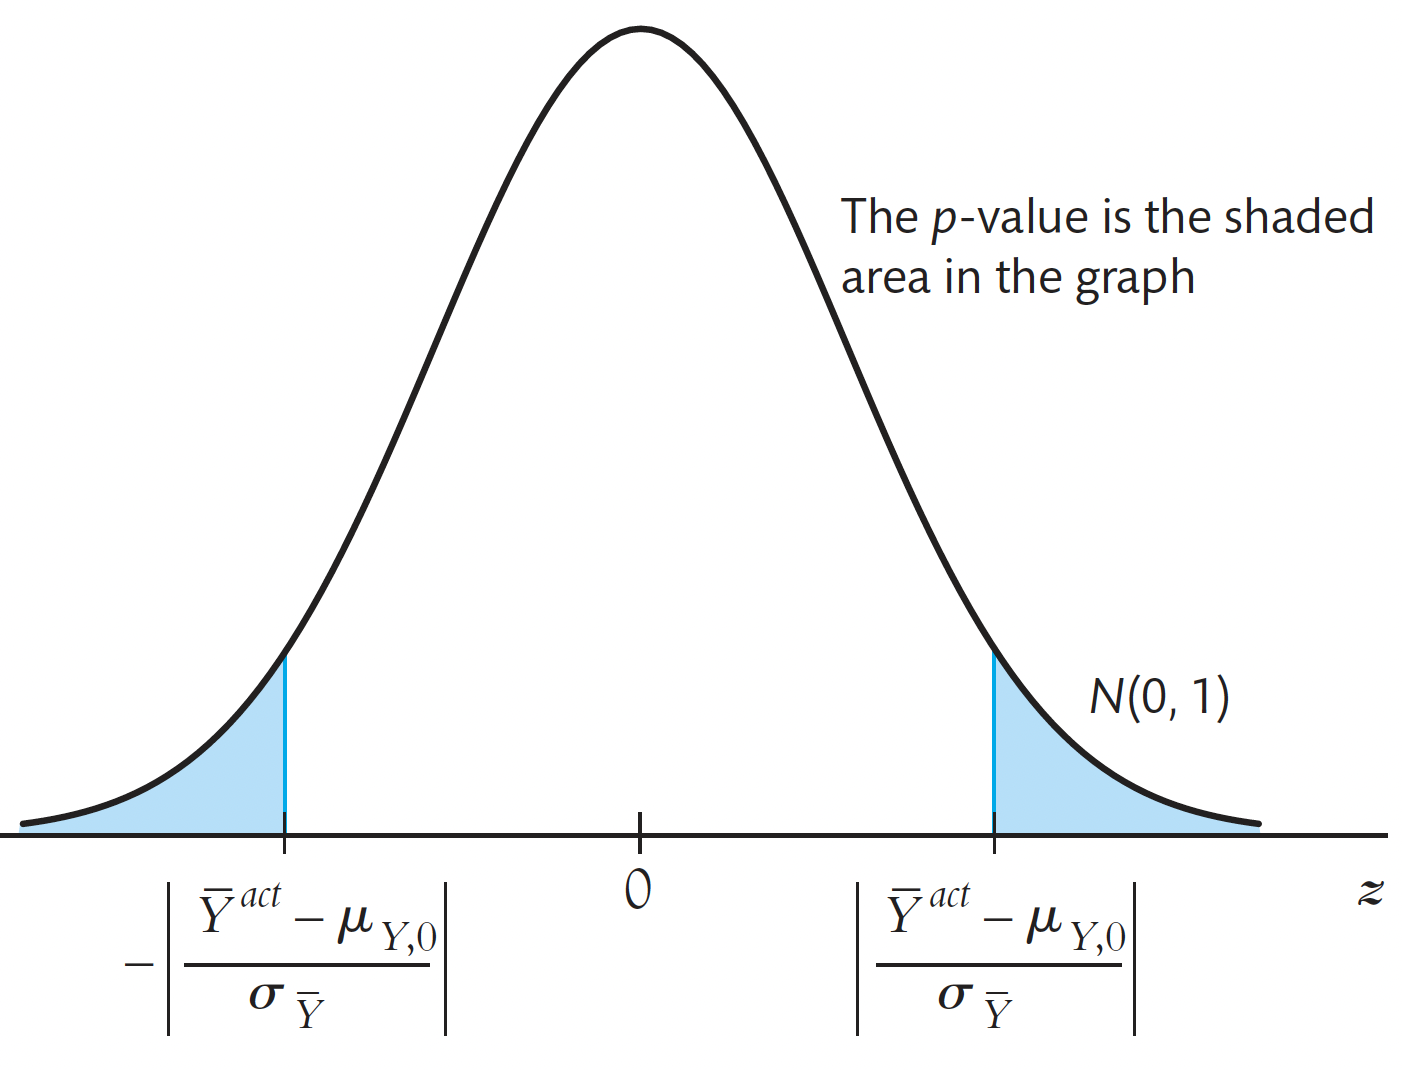
\includegraphics[scale=.3]{images/pvalue.png}
\end{figure}
\end{column}
\end{columns}
\end{frame}


\begin{frame}{Sample Variance and Sample Standard Deviation}
\begin{itemize}
    \item The sample variance, $s^2_Y$ is an estimator of the population variance $\sigma^2_Y$
    \begin{equation*}
        s^2_Y = \frac{1}{n-1}\sum_{i=1}^n (Y_i-\overline{Y})^2
    \end{equation*}
    \item The sample standard deviation, $s_Y = \sqrt{s^2_Y}$, is an estimator of the population standard deviation $\sigma_Y$
    \item There are two differences with the population variance, $\mathbb{E}[(Y-\mu_Y)^2]$:
    \begin{enumerate}
        \item $\mu_Y$ is unknown, so it is replaced by its natural estimator $\overline{Y}$
        \item We divide by $n-1$ (instead of $n$) to correct for the small downward bias generated by estimating $\mu_Y$ with $\overline{Y}$ (Bessel's correction)
    \end{enumerate}
    \item We can show that $s_Y^2 \xrightarrow{\mathit{p}}\sigma^2_Y$ as $n\rightarrow\infty$
\end{itemize}
\end{frame}

\begin{frame}{Standard Error to compute the p-value}
\begin{itemize}
    \item Because the variance of the sampling distribution, $\sigma_{\overline{Y}}^2 = \frac{\sigma_Y^2}{n}$, and sample variance is a consistent estimator of the population variance, $s_Y^2 \xrightarrow{\mathit{p}}\sigma^2_Y$, then $\frac{s_Y^2}{n} \xrightarrow{\mathit{p}}\frac{\sigma_Y^2}{n}=\sigma_{\overline{Y}}^2$
    \item In other words, the standard error, $SE(\overline{Y})=\hat{\sigma}_{\overline{Y}}=\frac{s_Y}{\sqrt{n}}$ is an estimator of the standard deviation of the sampling distribution of $\overline{Y}$
    \item Then, when $ \sigma_{\overline{Y}}$ is unknown because $\sigma_Y$ is unknown, one can still compute the p-value (under the assumption that $Y_1\dots Y_n$ are i.i.d.):
    \begin{equation*}
        \text{p-value} = 2\Phi\biggl(-\bigg| \frac{\overline{Y}^{act}-\mu_Y^0}{SE(\overline{Y})}\bigg|\biggl)
    \end{equation*}
    where the Standard Normal Cumulative Distribution Function, denoted as $\Phi(z)$, is a mathematical function that gives the probability that a standard normal random variable is less than or equal to a specific value $z$.

    \begin{equation*}
        \Phi(z) = \int_{-\infty}^{z} \frac{1}{\sqrt{2\pi}} e^{-x^2/2} \, dx
    \end{equation*}
\end{itemize}
\end{frame}


\begin{frame}{The t-statistic and its use for hypothesis testing}
\begin{itemize}
    \item The standardized sample average is called t-statistics, t-ratio, or Student's t-statistic.
    \begin{equation*}
        \text{t} = \frac{\overline{Y}-\mu_Y^0}{SE(\overline{Y})}
    \end{equation*}
    \item Because $s_Y^2 \xrightarrow{\mathit{p}}\sigma^2_Y$ as $n\rightarrow\infty$, then  $t\sim\mathcal{N}(0,1)$ as $n\rightarrow\infty$
    \item In general, we say we reject $H_0$ (or that $\overline{Y}$ is significantly different from $\mu_Y^0$) if the $\text{p-value}<.05$ (or when $\alpha=.01$)
    \item To summarize, testing $H^0$ against $H^1$ involves:
    \begin{enumerate}
        \item Compute the standard error of $\overline{Y}$, $SE(\overline{Y})$
        \item Compute the corresponding t-statistic
        \item Compute the p-value. Reject $H^0$ at the 5\% significance level if the p-value is less than 0.05 (or alternatively, if $\mid t^{act} \mid > 1.96$)
    \end{enumerate}
    \item But what are the consequences of making errors in hypothesis testing?
\end{itemize}
\end{frame}

\begin{frame}[shrink=5]
    \frametitle{Type I and Type II Errors in Hypothesis Testing}

    \begin{exampleblock}{Type I Error (False Positive)}
        \begin{itemize}
            \item Occurs when we reject a null hypothesis that is actually true.
            \item Denoted as $\alpha$ (alpha), the chosen significance level.
            \item Probability of Type I Error: $\alpha$.
            \item Example: Incorrectly concluding a drug is effective when it's not.
            \item Consequence: Often considered more serious due to potential harm.
        \end{itemize}
    \end{exampleblock}

    \begin{exampleblock}{Type II Error (False Negative)}
        \begin{itemize}
            \item Occurs when we fail to reject a null hypothesis that is actually false.
            \item Denoted as $\beta$ (beta).
            \item Probability of Type II Error: Influenced by factors like sample size, effect size, and $\alpha$.
            \item Example: Failing to detect a real positive effect of a drug.
            \item Consequence: May result in missed opportunities for important discoveries or interventions.
        \end{itemize}
    \end{exampleblock}

    In hypothesis testing, the choice of $\alpha$ and sample size affects the balance between Type I and Type II errors.
\end{frame}



\begin{frame}{Errors in Hypothesis Testing}
\begin{figure}
  \centering
         \vspace{-1mm}
        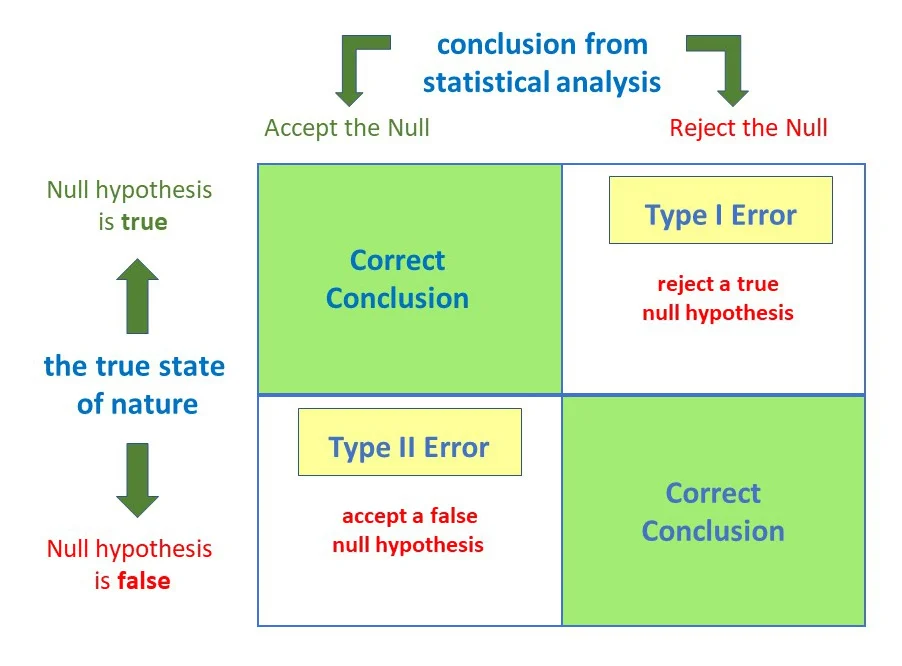
\includegraphics[scale=.33]{images/errortypes1.png}
\end{figure}
\end{frame}

\begin{frame}{$H^0$: Patient is \textit{not} pregnant | $H^1$: Patient is pregnant}
\begin{figure}
  \centering
         \vspace{-1mm}
        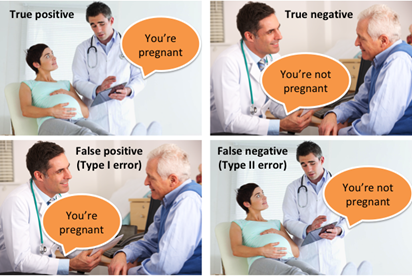
\includegraphics[scale=.9]{images/errortypes2.png}
\end{figure}
\end{frame}

\begin{frame}
    \frametitle{What are Confidence Intervals (CIs)?}
    
    \begin{exampleblock}{Definition}
        A Confidence Interval (CI) is a range of values constructed from sample data that is likely to contain the true population parameter with a certain level of confidence.
    \end{exampleblock}
    
    \begin{block}{Example}
        If we estimate the average height of a population to be 170 cm with a 95\% CI to be (165 cm, 175 cm), it means we are 95\% confident that the true average height falls within this interval.
    \end{block}
    \begin{itemize}
        \item They provide a range of plausible values for a population parameter, not just a single point estimate.
        \item CIs help us quantify the uncertainty in our estimates.
        \item CIs help us make informed decisions in the presence of uncertainty.
        \item They are widely used in research, business, and policy to convey the reliability of estimates.
    \end{itemize}
    
\end{frame}


\begin{frame}{Computing CIs}
%A 95\% two-sided confidence interval for $\mu_Y$ is an interval constructed so that it contains the true value of $\mu_Y$ in 95\% of all possible random samples. When the sample size n is large, 90\%, 95\%, and 99\% confidence intervals for $\mu_Y$ are:
\begin{itemize}
    \item 90\% confidence interval for $\mu_Y$  =$\overline{Y}\pm 1.64 \times SE(\overline{Y})$
    \item 95\% confidence interval for $\mu_Y$  =$\overline{Y}\pm 1.96 \times SE(\overline{Y})$
    \item 99\% confidence interval for $\mu_Y$  =$\overline{Y}\pm 2.58 \times SE(\overline{Y})$
\end{itemize}

\begin{block}{Example}
\begin{itemize}
    \item You collect a random sample of $n=50$ individuals at UPF and measure their heights. The sample mean height, $\overline{Y}$, is 170 cm, and the sample standard deviation, $s_Y$, is 8 cm.
    \item The standard error, $SE(\overline{Y}),$ is $\frac{8}{\sqrt{50}}$
    \item The 95\% confidence interval is given by
    \begin{equation*}
        170 \pm 1.96 \times \frac{8}{\sqrt{50}} \approx [167.78 ; 172.22]
    \end{equation*}
    \item We are 95\% confident that the true average height of adults at UPF falls within the interval [167.78 ; 172.22]
\end{itemize}
\end{block}
\end{frame}


\begin{frame}{Mean Difference Testing: Comparing Groups 1/2}
\begin{itemize}
    \item Consider the null hypothesis that mean earnings for these two populations differ by a certain amount, say, $d_0$
    \begin{equation*}
        H^0: \mu_Y^a - \mu_Y^b = d_0 \textbf{~~~vs~~~} H^1: \mu_Y^a - \mu_Y^b \neq d_0
    \end{equation*}
    \item In a lot of applied studies $d_0=0$, which means
        \begin{equation*}
        H^0: \mu_Y^a = \mu_Y^b \textbf{~~~vs~~~} H^1: \mu_Y^a \neq \mu_Y^b
    \end{equation*}
    \item You have computed $\overline{Y}^a$ and $\overline{Y}^b$. From there, derive the sample variance $var(\overline{Y}^a-\overline{Y}^b)$ and deduce the $SE(\mu_Y^a - \mu_Y^b)$
    \begin{eqnarray*}
       &var((\overline{Y}^a - \overline{Y}^b) - d_0) &=   var(\overline{Y}^a) +  var(\overline{Y}^b) - 2cov(\overline{Y}^a ,\overline{Y}^b)\\
       \Rightarrow &SE(\overline{Y}^a - \overline{Y}^b - d_0) &=\sqrt{\frac{var(\overline{Y}^a)}{n}+\frac{var(\overline{Y}^b)}{n}} 
    \end{eqnarray*}

\end{itemize}
\end{frame}


\begin{frame}{Mean Difference Testing: Comparing Groups 2/2}
\begin{itemize}
    \item Once we have $SE((\mu_Y^a - \mu_Y^b)  - d_0)$, we can easily compute the corresponding t-statistic
    \begin{equation*}
        t = \frac{(\overline{Y}^a - \overline{Y}^b) - d_0}{SE((\overline{Y}^a - \overline{Y}^b)  - d_0)}
    \end{equation*}
    \item[$\rightarrow$] We can reject that $\mu_Y^a - \mu_Y^b = d_0$ at the 5\%-level when $\mid t \mid > 1.96$ \vspace{.5cm}
    \item Similarly, we can construct the confidence interval for $\mu_Y^a - \mu_Y^b=d_0$
    \begin{equation*}
        CI_{\mu_Y^a - \mu_Y^b=d_0} = (\overline{Y}^a -\overline{Y}^b)+1.96\times SE((\overline{Y}^a - \overline{Y}^b)  - d_0)
    \end{equation*}
    \item[$\rightarrow$] We can reject that $\mu_Y^a - \mu_Y^b = d_0$ at the 5\%-level when $d_0\notin CI_{\mu_Y^a - \mu_Y^b=d_0}$\vspace{.5cm}
    \item Comparing mean differences is very useful, e.g., when one wants to verify that control and treatment groups are comparable in means before receiving treatment (i.e., balance tests).
\end{itemize}
\end{frame}

\begin{frame}{Causal Inference in Randomized Control Trials}
\begin{itemize}
    \item In the ideal, golden standard RCT case, the causal effect of a treatment variable $D$ on an outcome variable $Y$ is the difference in conditional expectations; i.e., for a dummy treatment,
    \begin{equation*}
        \mathbb{E}(Y\mid D=1)-\mathbb{E}(Y\mid D=0)
    \end{equation*}
    \item The randomized assignment of the treatment helps ensure that any observed differences are likely due to the intervention, reducing confounding.
    \item Mean Difference Testing allows us to test whether $\mathbb{E}(Y\mid D=1)= \mathbb{E}(Y\mid D=0)$
    \item Example 1: Drug Efficacy
        \begin{itemize}
            \item Treatment Group: Receives the new drug.
            \item Control Group: Receives a placebo.
            \item Mean Difference Testing helps determine if the drug has a significant effect on health outcomes.
        \end{itemize}
    \item Example 2: Educational Interventions
        \begin{itemize}
            \item Different teaching methods in classrooms.
            \item Mean Difference Testing assesses if one method leads to better student performance.
        \end{itemize}
\end{itemize}
\end{frame}


\begin{frame}{The California Test Score Data Set}
 \begin{columns}
\begin{column}{0.35\textwidth}
    \begin{itemize}
    \item All K-6 and K-8 California school districts ($n=500$) (CPS, 1999)
    \item Test score: sum of math and English/language arts, 5th grade
    \item Subsidized Meals: free or reduced-price meals
    \end{itemize}
\end{column}
\begin{column}{0.7\textwidth}
\begin{figure}
  \centering
         \vspace{-1mm}
        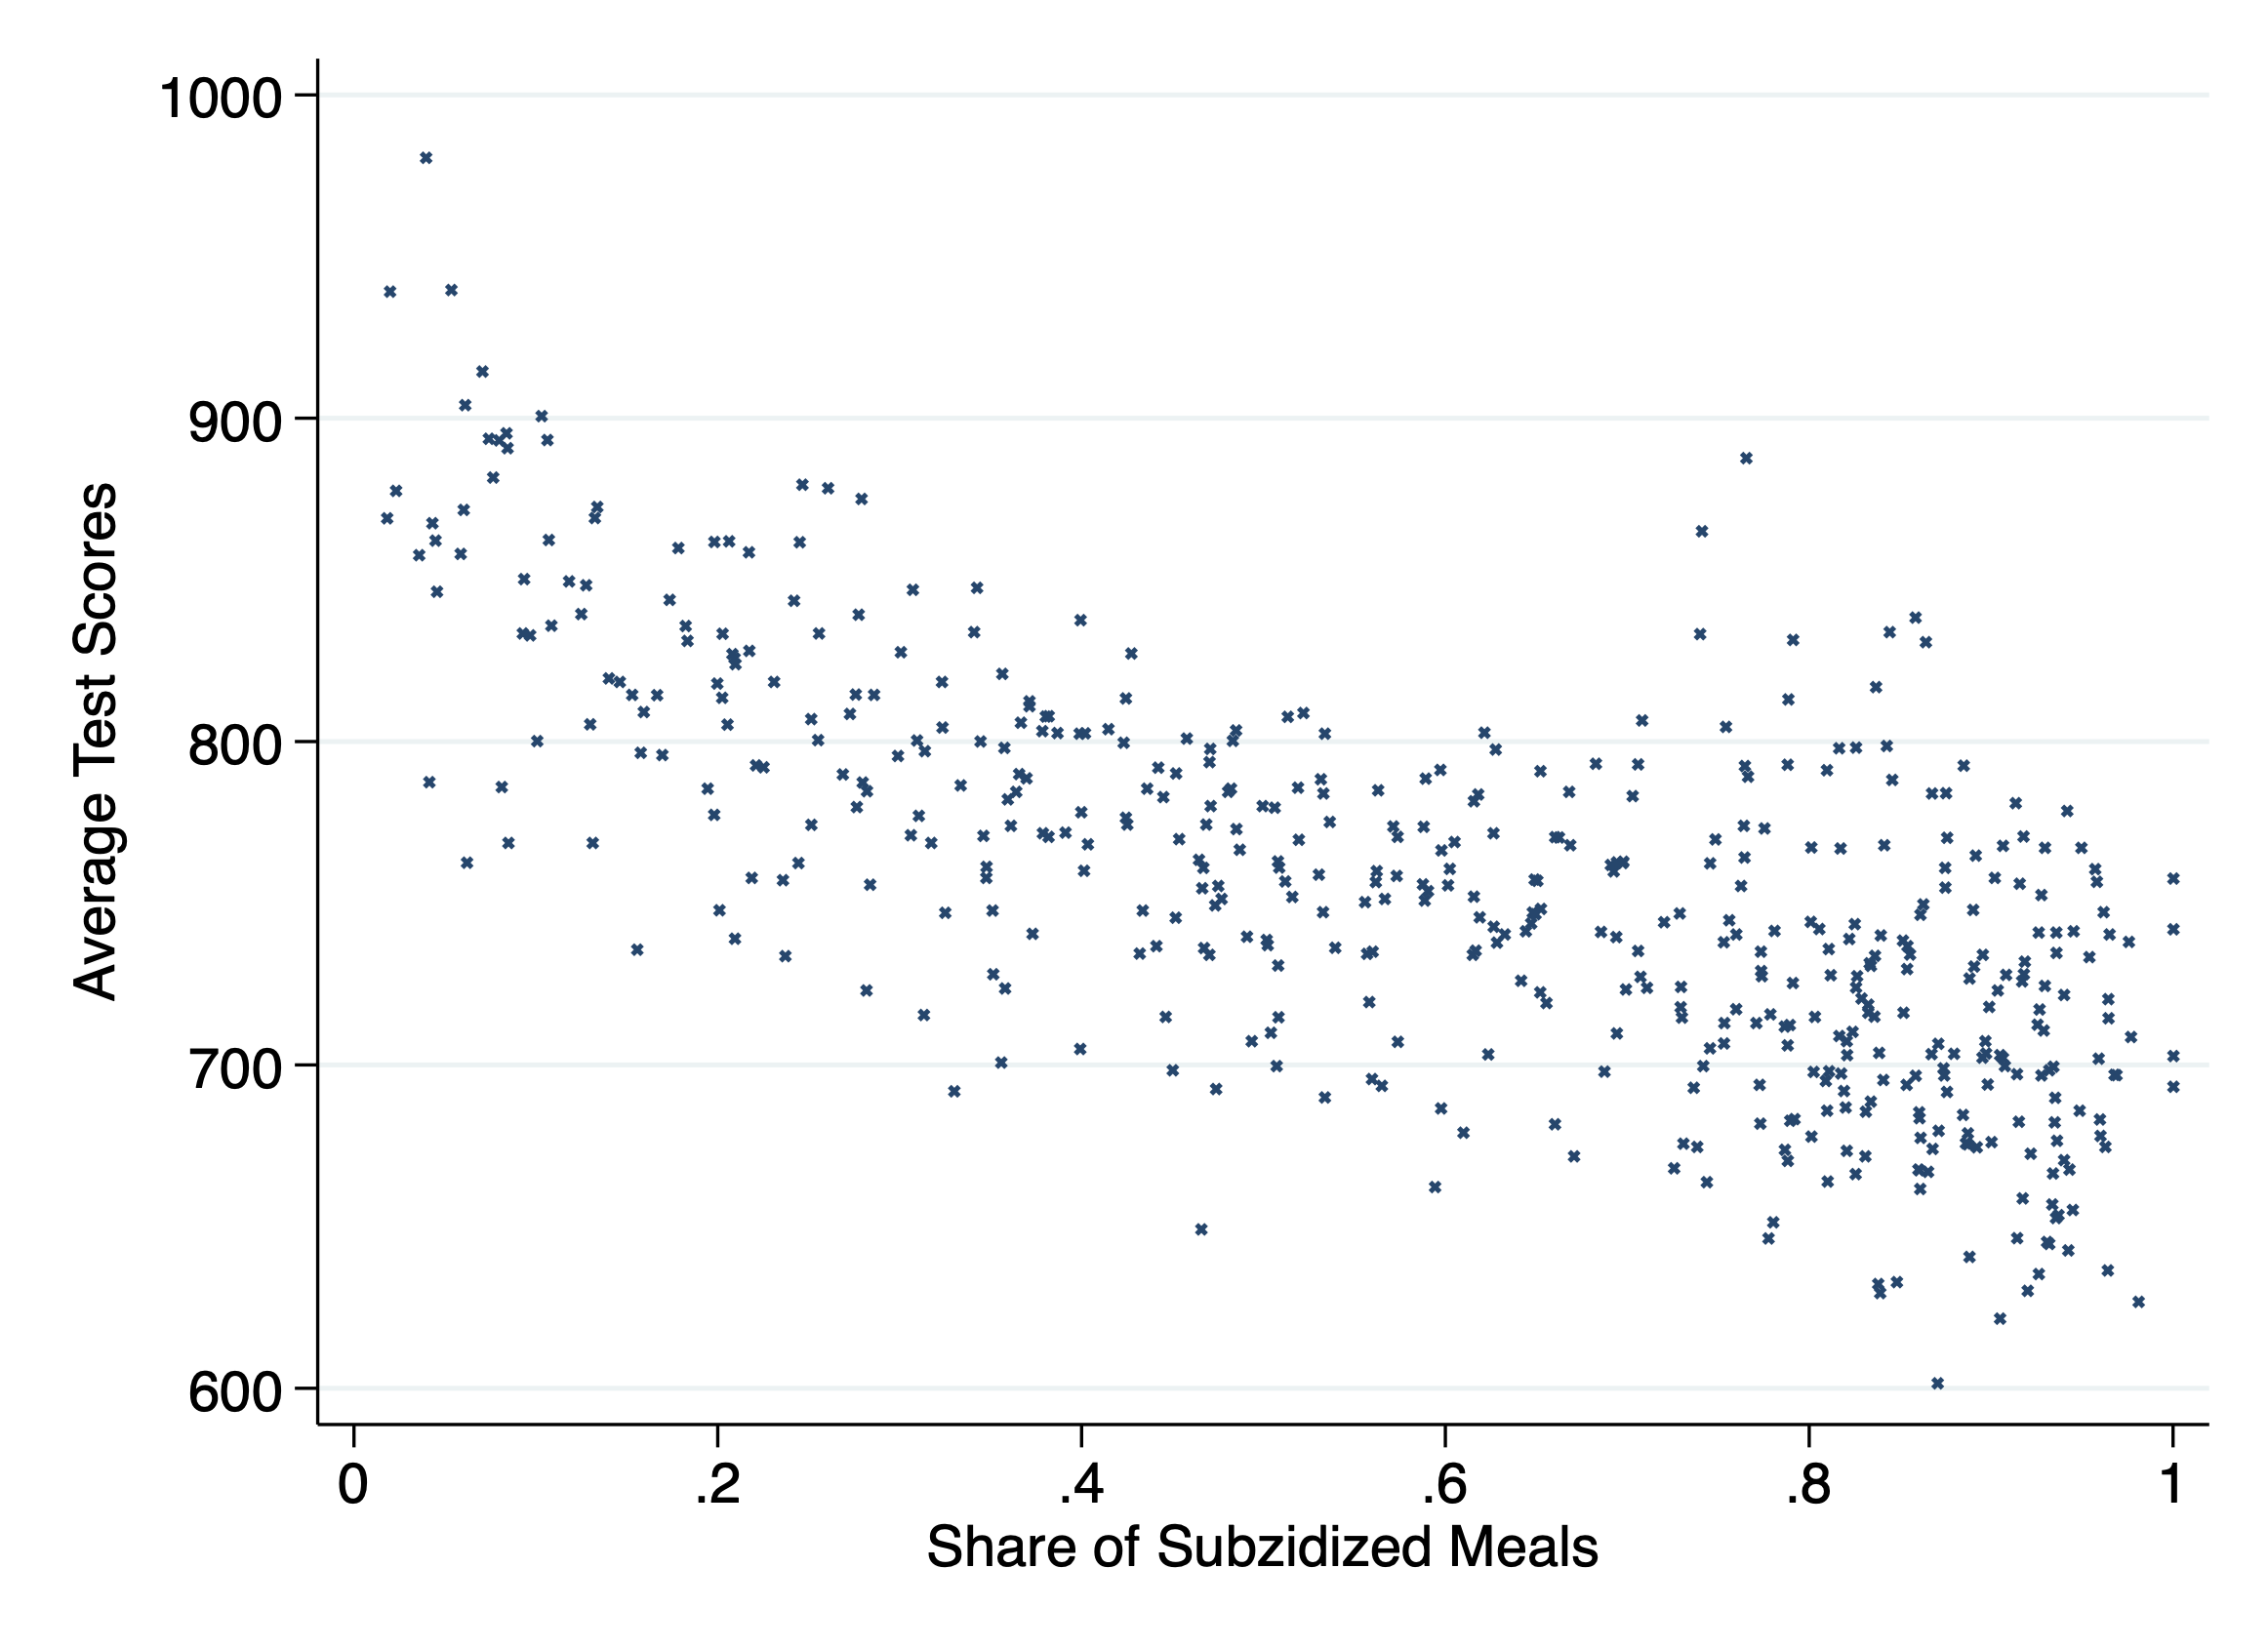
\includegraphics[scale=.25]{images/testscores_scatter.png}
\end{figure}
\end{column}
\end{columns}
\end{frame}

\begin{frame}{The California Test Score Data Set}
The scatter plot does not tell us much about each variable, independently. We can provide descriptive statistics of the sample:
\begin{table}[]
\begin{tabular}{l|c|c|c|c|c|}
\cline{2-6}
\textit{}                                                & Median & p25    & p75    & Min   & Max  \\ \hline
\multicolumn{1}{|l|}{\textit{Test Scores}}                & 751.5  & 708.95 & 791.75 & 601.7 & 980.7  \\ \hline
\multicolumn{1}{|l|}{\textit{Share of Subsidized Meals}} & .6511  & .3755  & .8432  & .018  & 1    \\ \hline
\end{tabular}
\end{table}

\begin{table}[]
\begin{tabular}{l|c|c|c|c|}
\cline{2-5}
\textit{}                                               & Mean     & sd       & Skewness & Kurtosis \\ \hline
\multicolumn{1}{|l|}{\textit{Test Scores}}               & 753.8542 & 60.3035  & .3696458 & 3.150585 \\ \hline
\multicolumn{1}{|l|}{\textit{Share of Subsidized Meals}}   & .6018114 & .2758199 & -.445432 & 1.958609 \\ \hline
\end{tabular}
\end{table}


\end{frame}

\begin{frame}{The California Test Score Data Set}
 \begin{columns}
\begin{column}{0.35\textwidth}
    \begin{itemize}
    \item This allows us to study the joint distribution of the \textit{Test Scores} and the \textit{Share of Subsidized Meals}
    \item We can compute the sample covariance, $s_{XY} = \frac{1}{n-1}\sum^n_{i=1} (X_i-\overline{X})(Y_i-\overline{Y})$
    \item Here, $s_{XY} = -11.7839$
    \item The sample correlation, $r_{XY} = \frac{s_{XY}}{s_{X}s_{Y}}$
    \item Here, $r_{XY} \approx \frac{-11.78}{60.3\times0.28} \approx -.7$
    \end{itemize}
\end{column}
\begin{column}{0.7\textwidth}
\begin{figure}
  \centering
         \vspace{-1mm}
        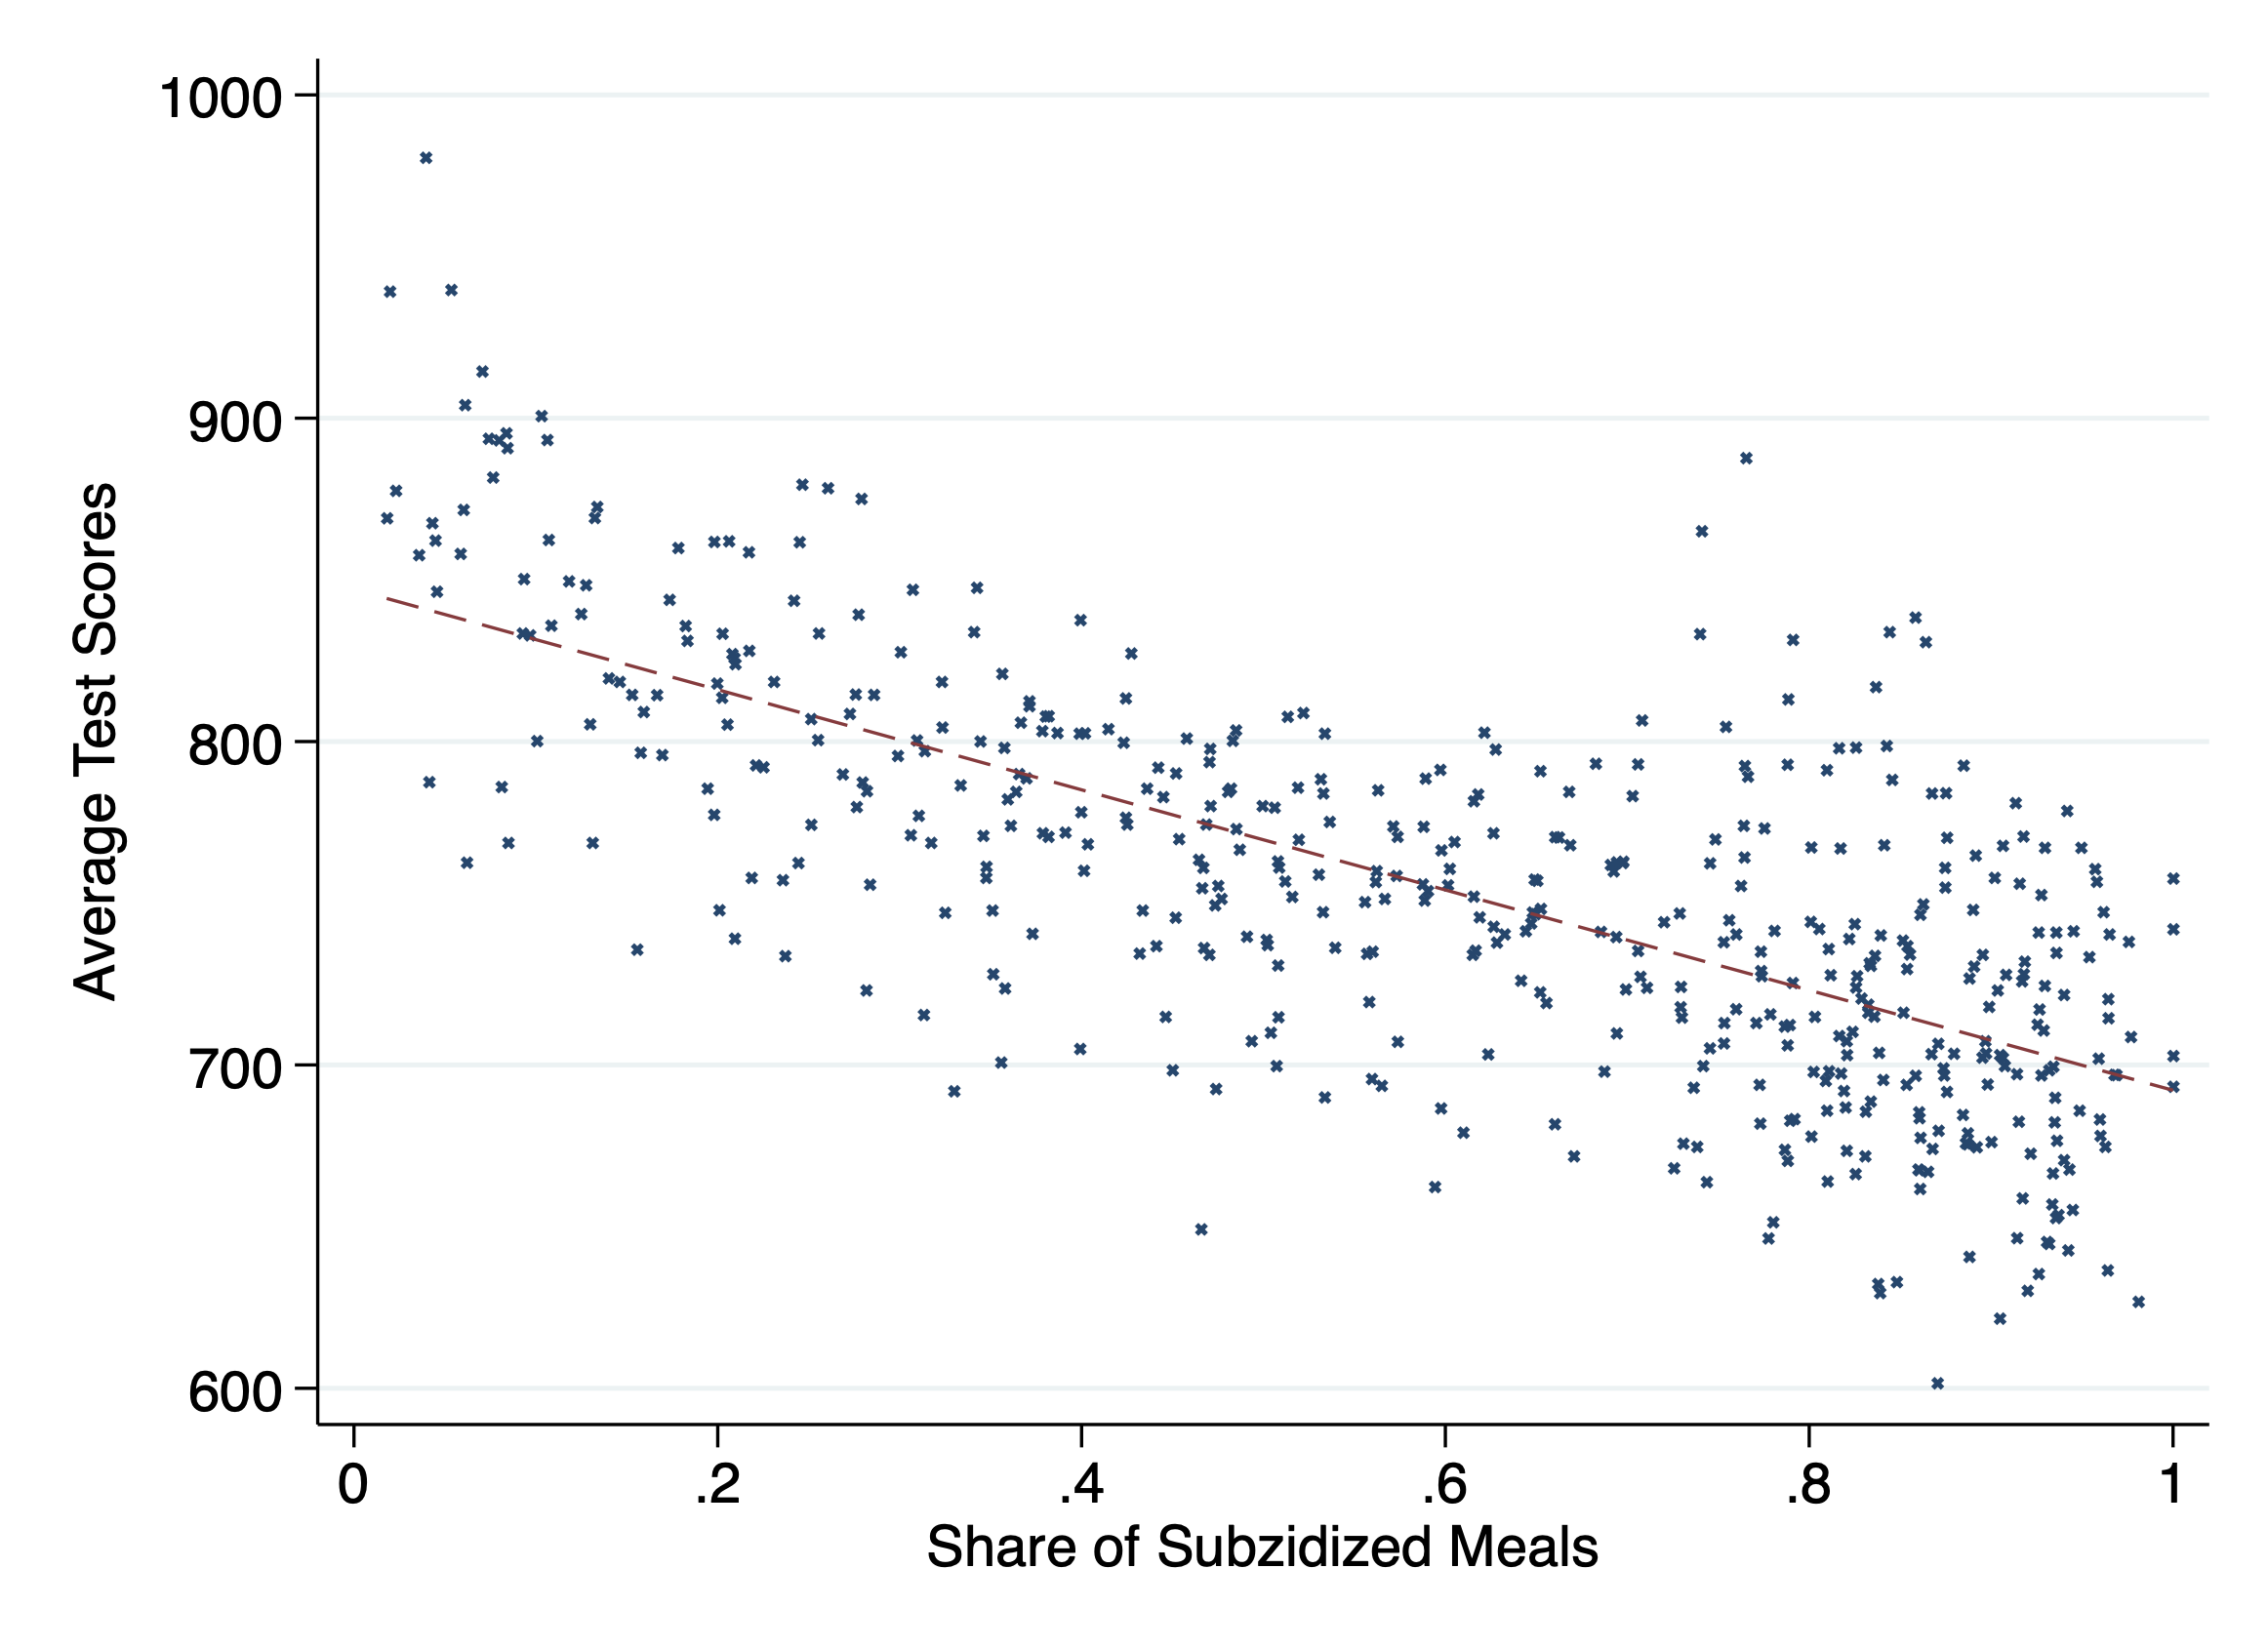
\includegraphics[scale=.25]{images/testscores_corr.png}
\end{figure}
\end{column}
\end{columns}
\end{frame}


\begin{frame}{The California Test Score Data Set}
 \begin{columns}
\begin{column}{0.35\textwidth}
    \begin{itemize}
    \item Are schools with less subsidized meals significantly better than schools with more subsidized meals?
    \item We can split the distribution into two groups:
    \begin{enumerate}
        \item Below-median \textit{Share of Subsidized Meals} (red)
        \item Above-median \textit{Share of Subsidized Meals} (red)
    \end{enumerate}
    \end{itemize}
\end{column}
\begin{column}{0.7\textwidth}
\begin{figure}
  \centering
         \vspace{-1mm}
        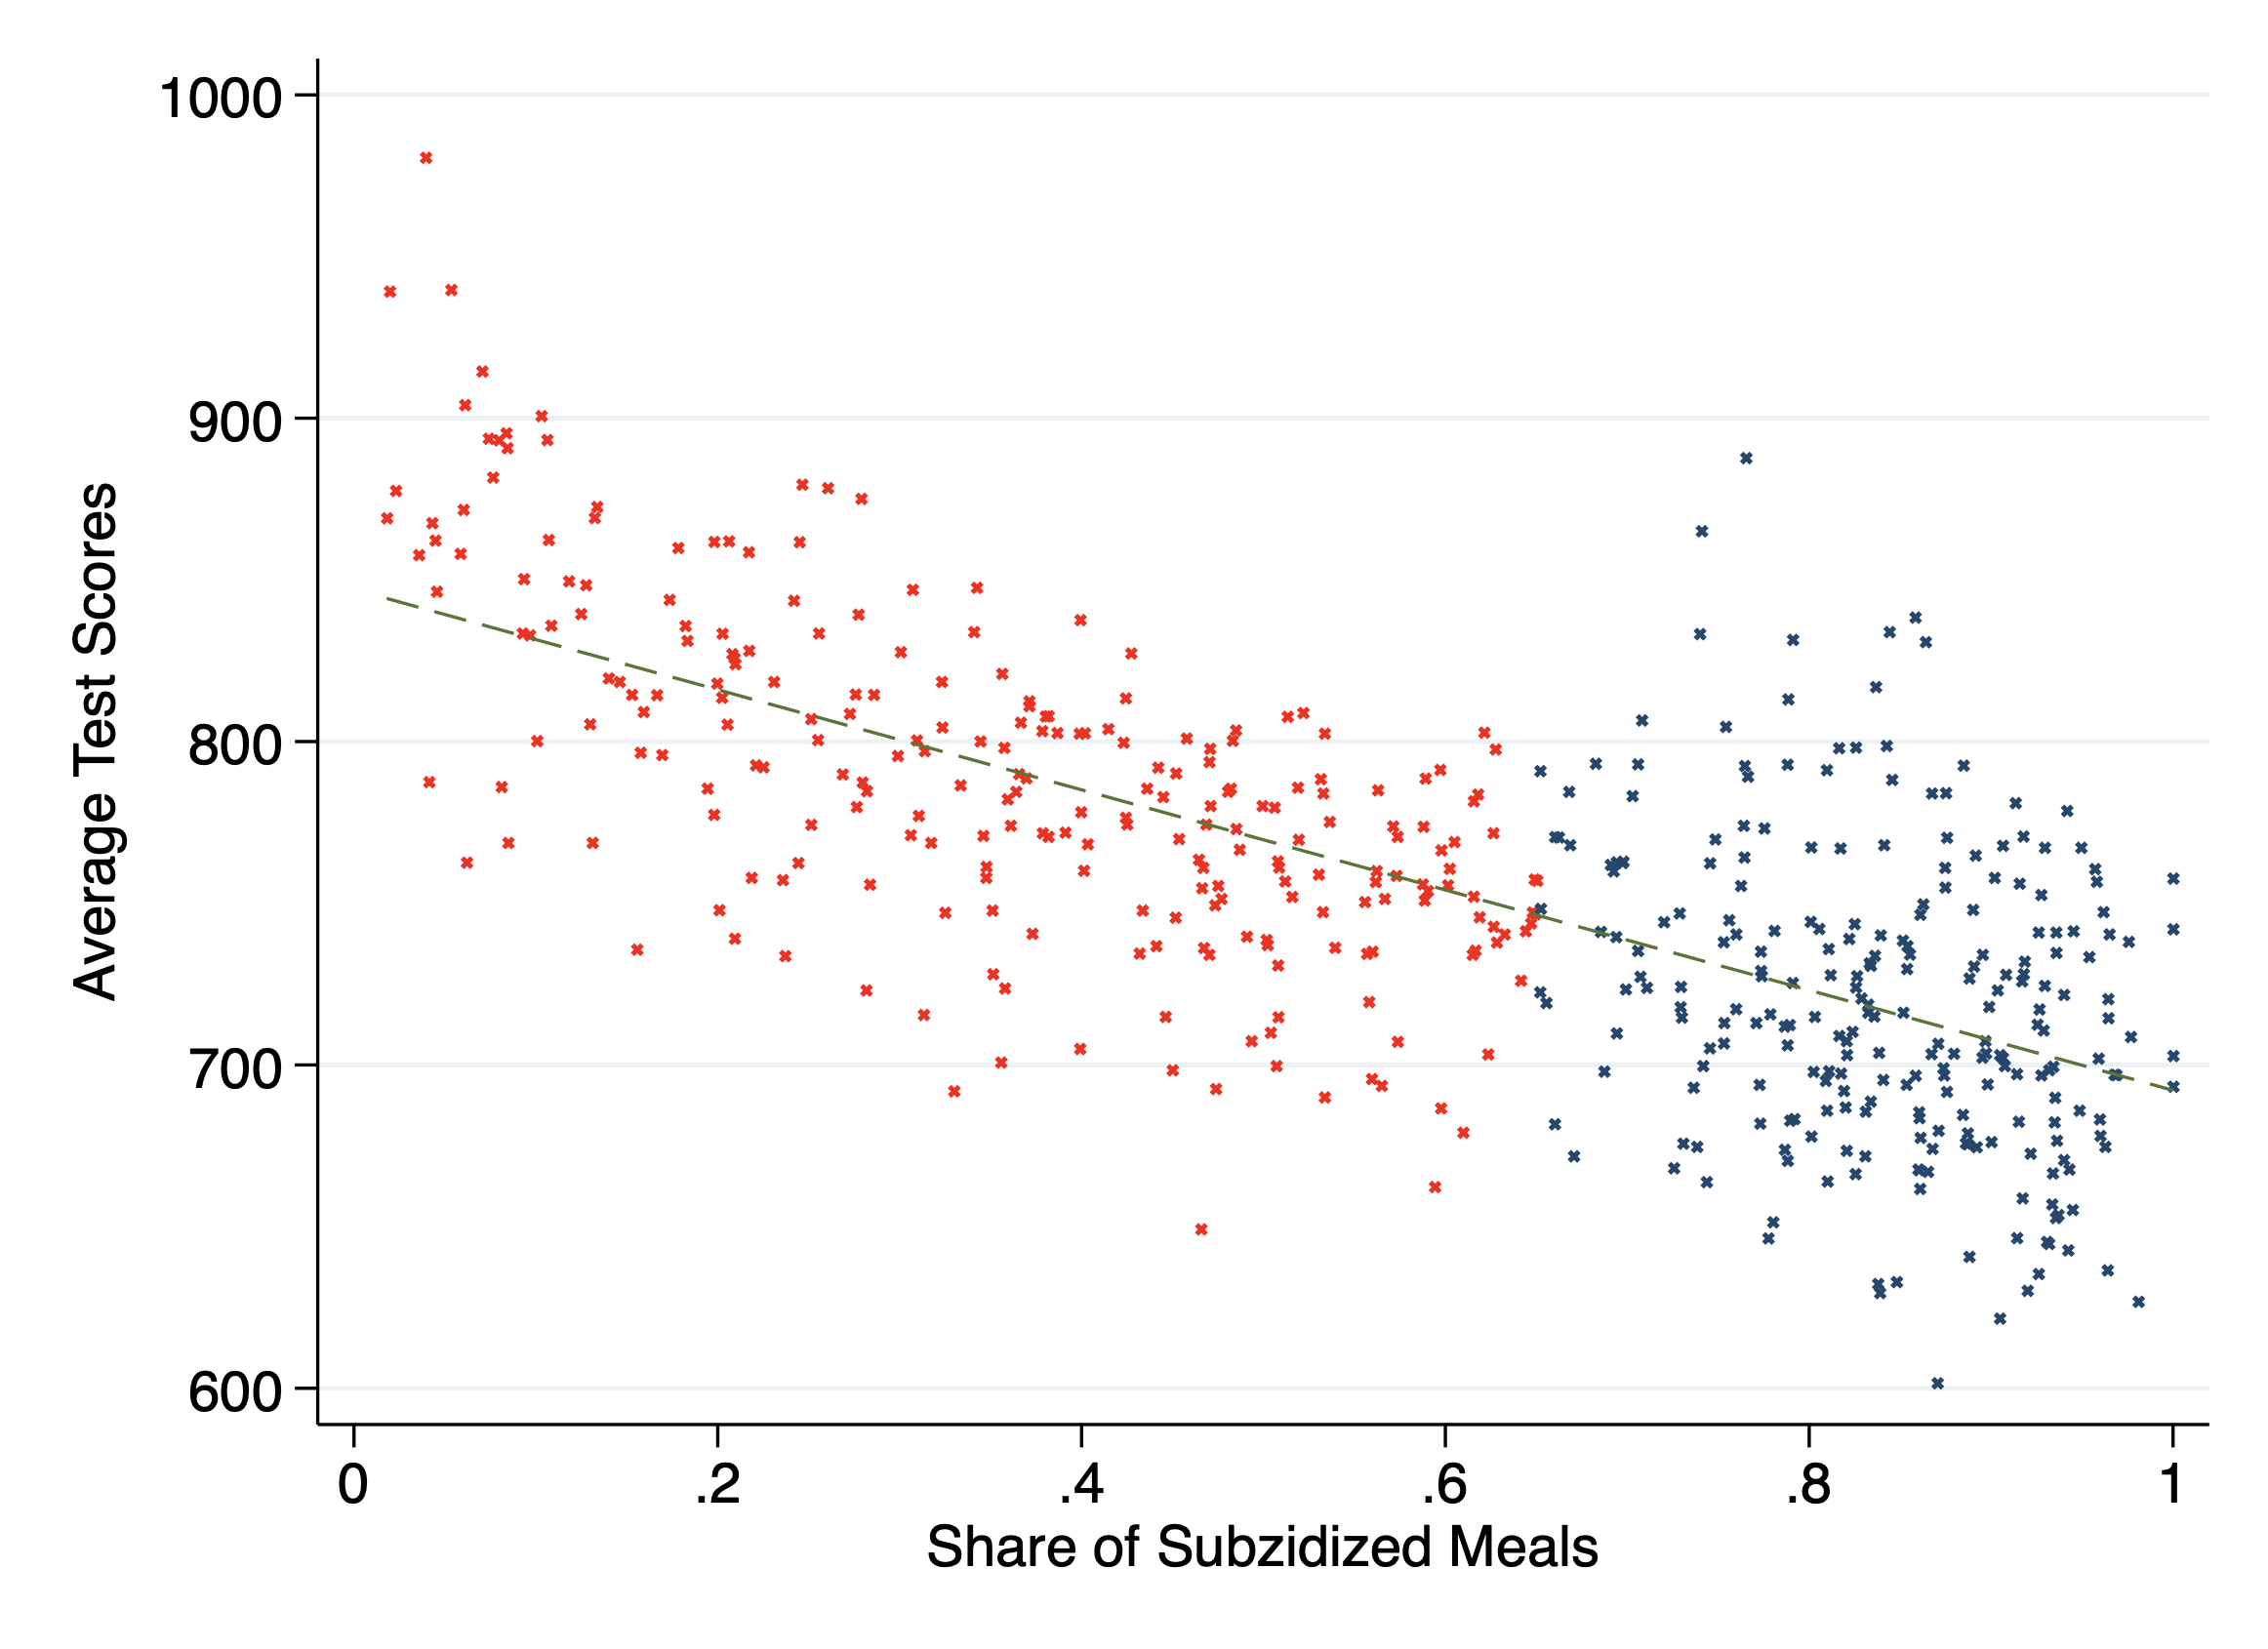
\includegraphics[scale=.25]{images/testscores_group1.png}
\end{figure}
\end{column}
\end{columns}
\end{frame}

\begin{frame}{The California Test Score Data Set}
 \begin{columns}
\begin{column}{0.35\textwidth}
Estimation:
    \begin{itemize}
    \item Compare average test scores in districts with low \textit{Share of Subsidized Meals} to those with high \textit{Share of Subsidized Meals}
    \end{itemize}
\end{column}
\begin{column}{0.7\textwidth}
\begin{figure}
  \centering
         \vspace{-1mm}
        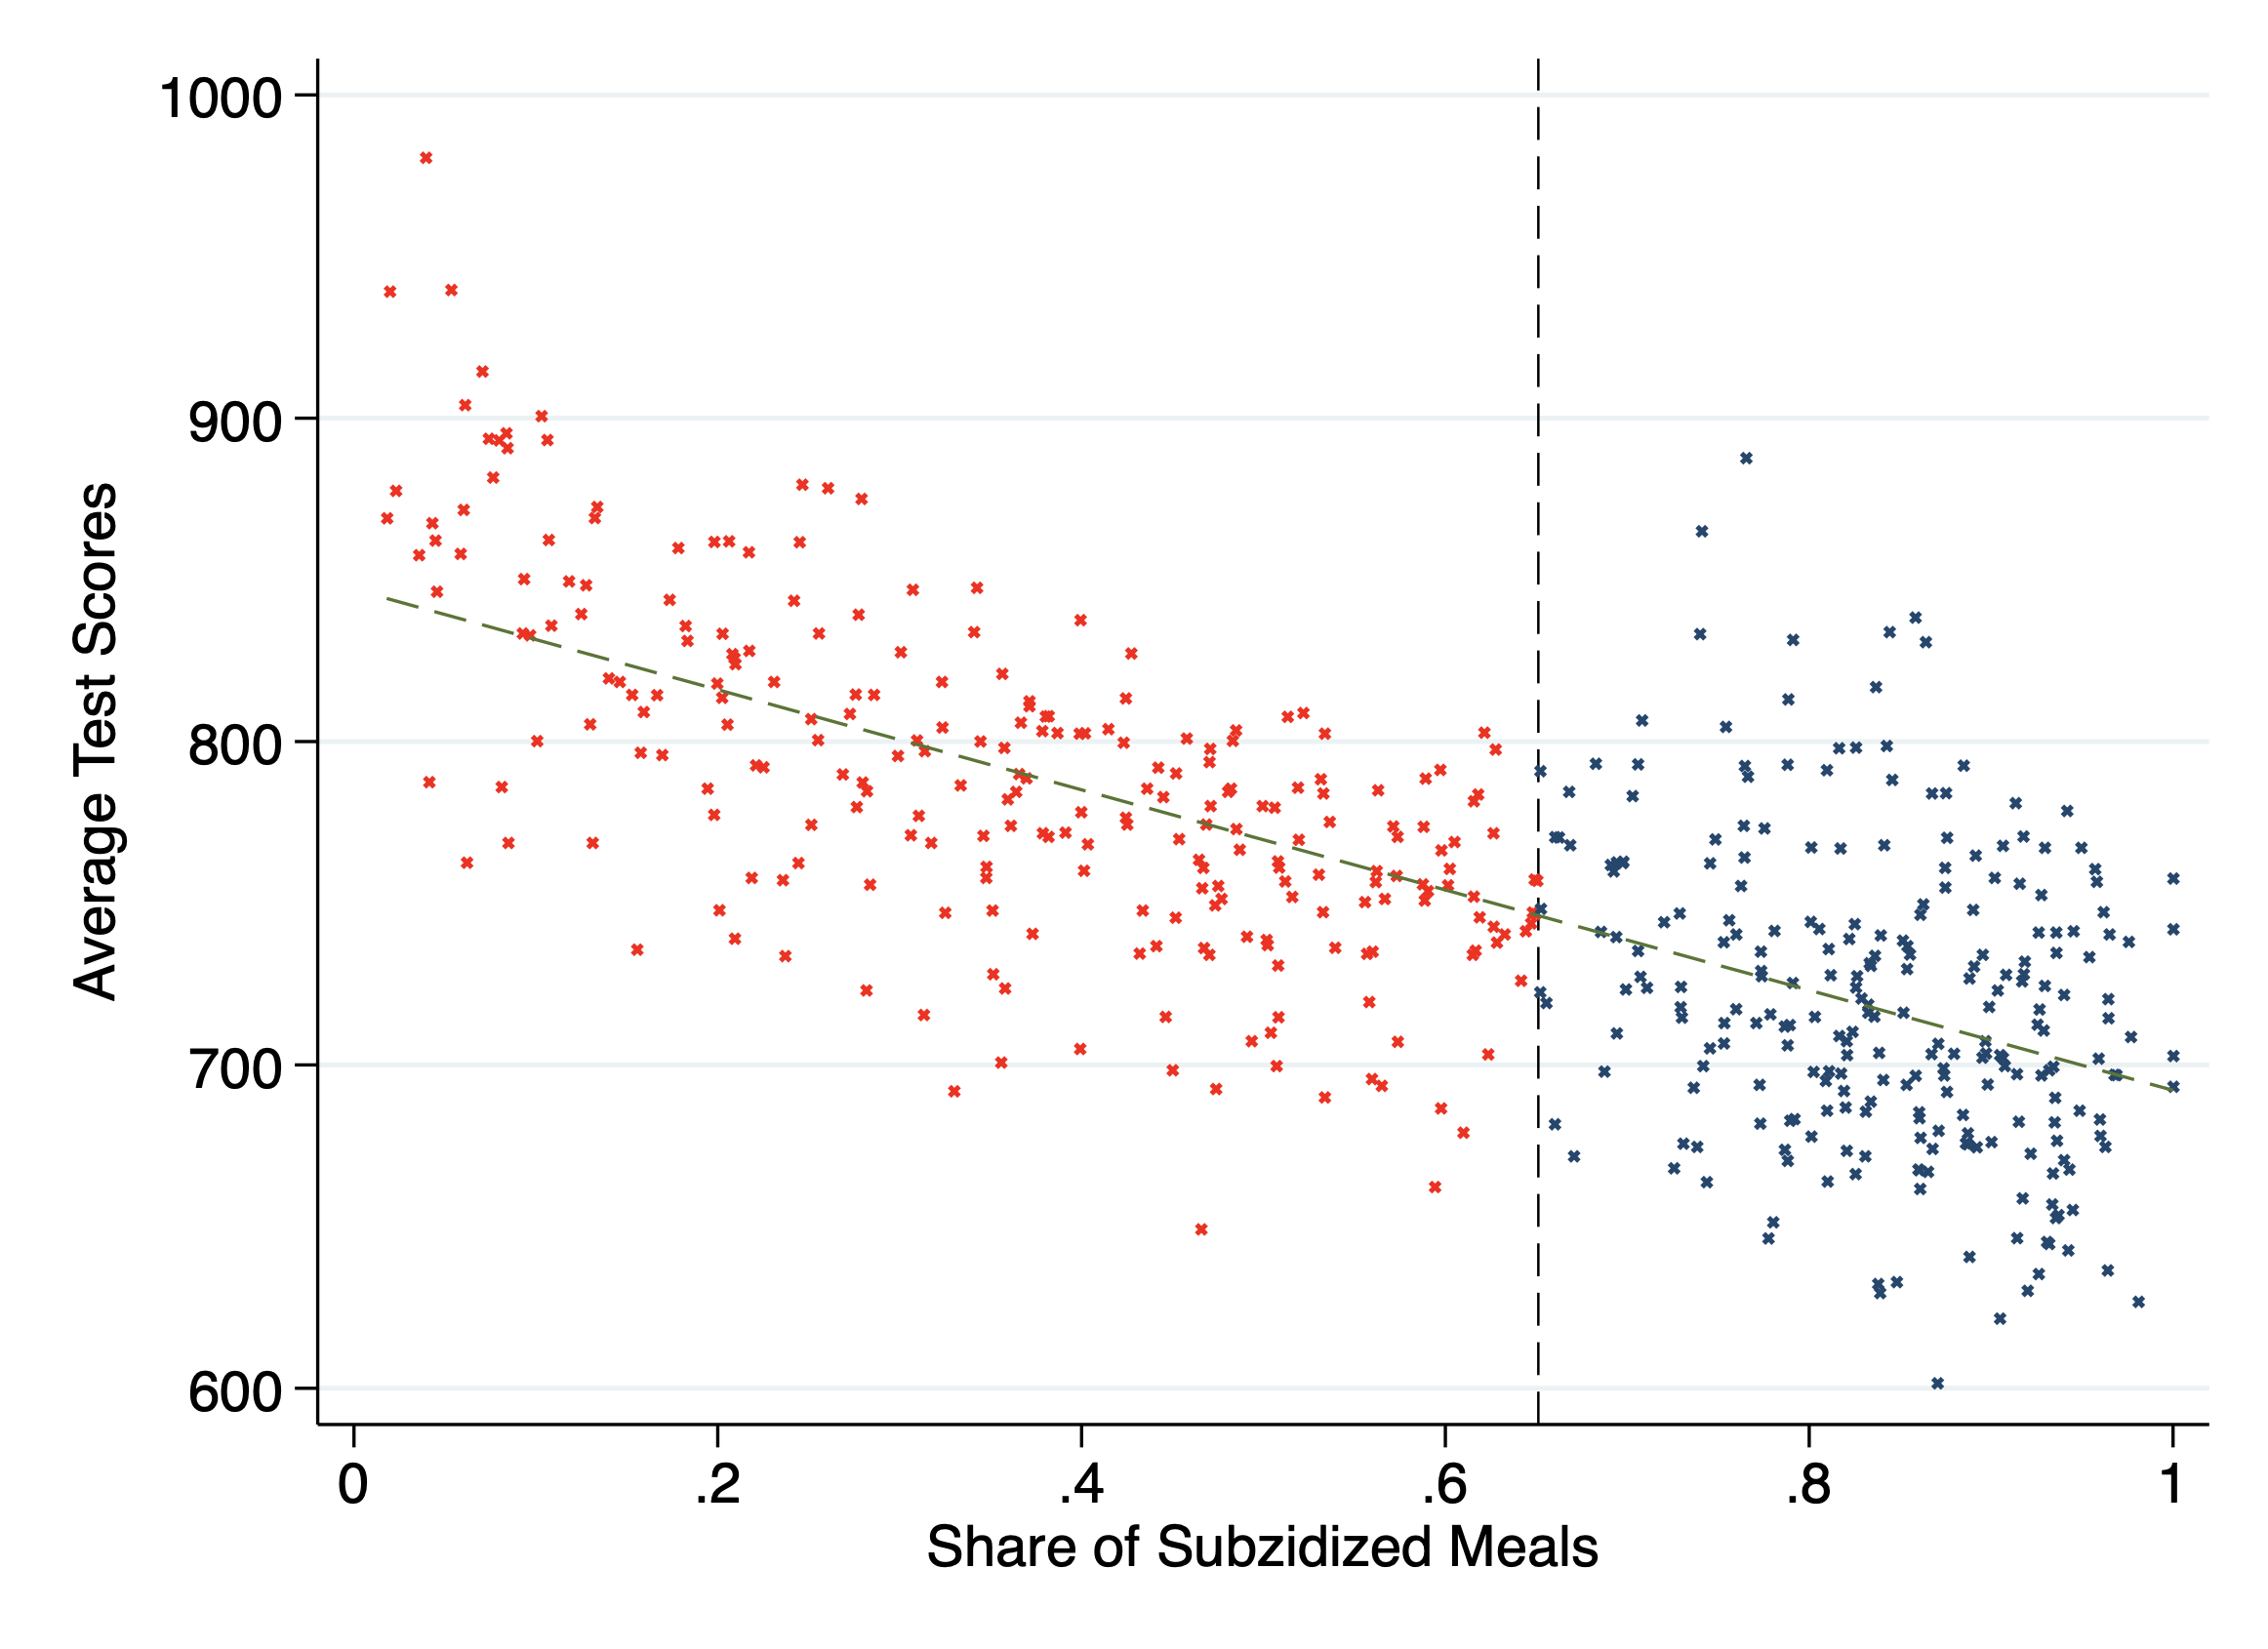
\includegraphics[scale=.25]{images/testscores_group2.png}
\end{figure}
\end{column}
\end{columns}
\end{frame}

\begin{frame}{The California Test Score Data Set}
 \begin{columns}
\begin{column}{0.35\textwidth}
Hypothesis testing:
    \begin{itemize}
    \item Test the “null” hypothesis that the mean test scores in the two types of groups are the same, against the “alternative” hypothesis that they differ 
    \item $H^0: \overline{Y}^{X^L} - \overline{Y}^{X^H} = 0 $
    \item $H^1: \overline{Y}^{X^L} - \overline{Y}^{X^H} \neq 0 $
    \end{itemize}
\end{column}
\begin{column}{0.7\textwidth}
\begin{figure}
  \centering
         \vspace{-1mm}
        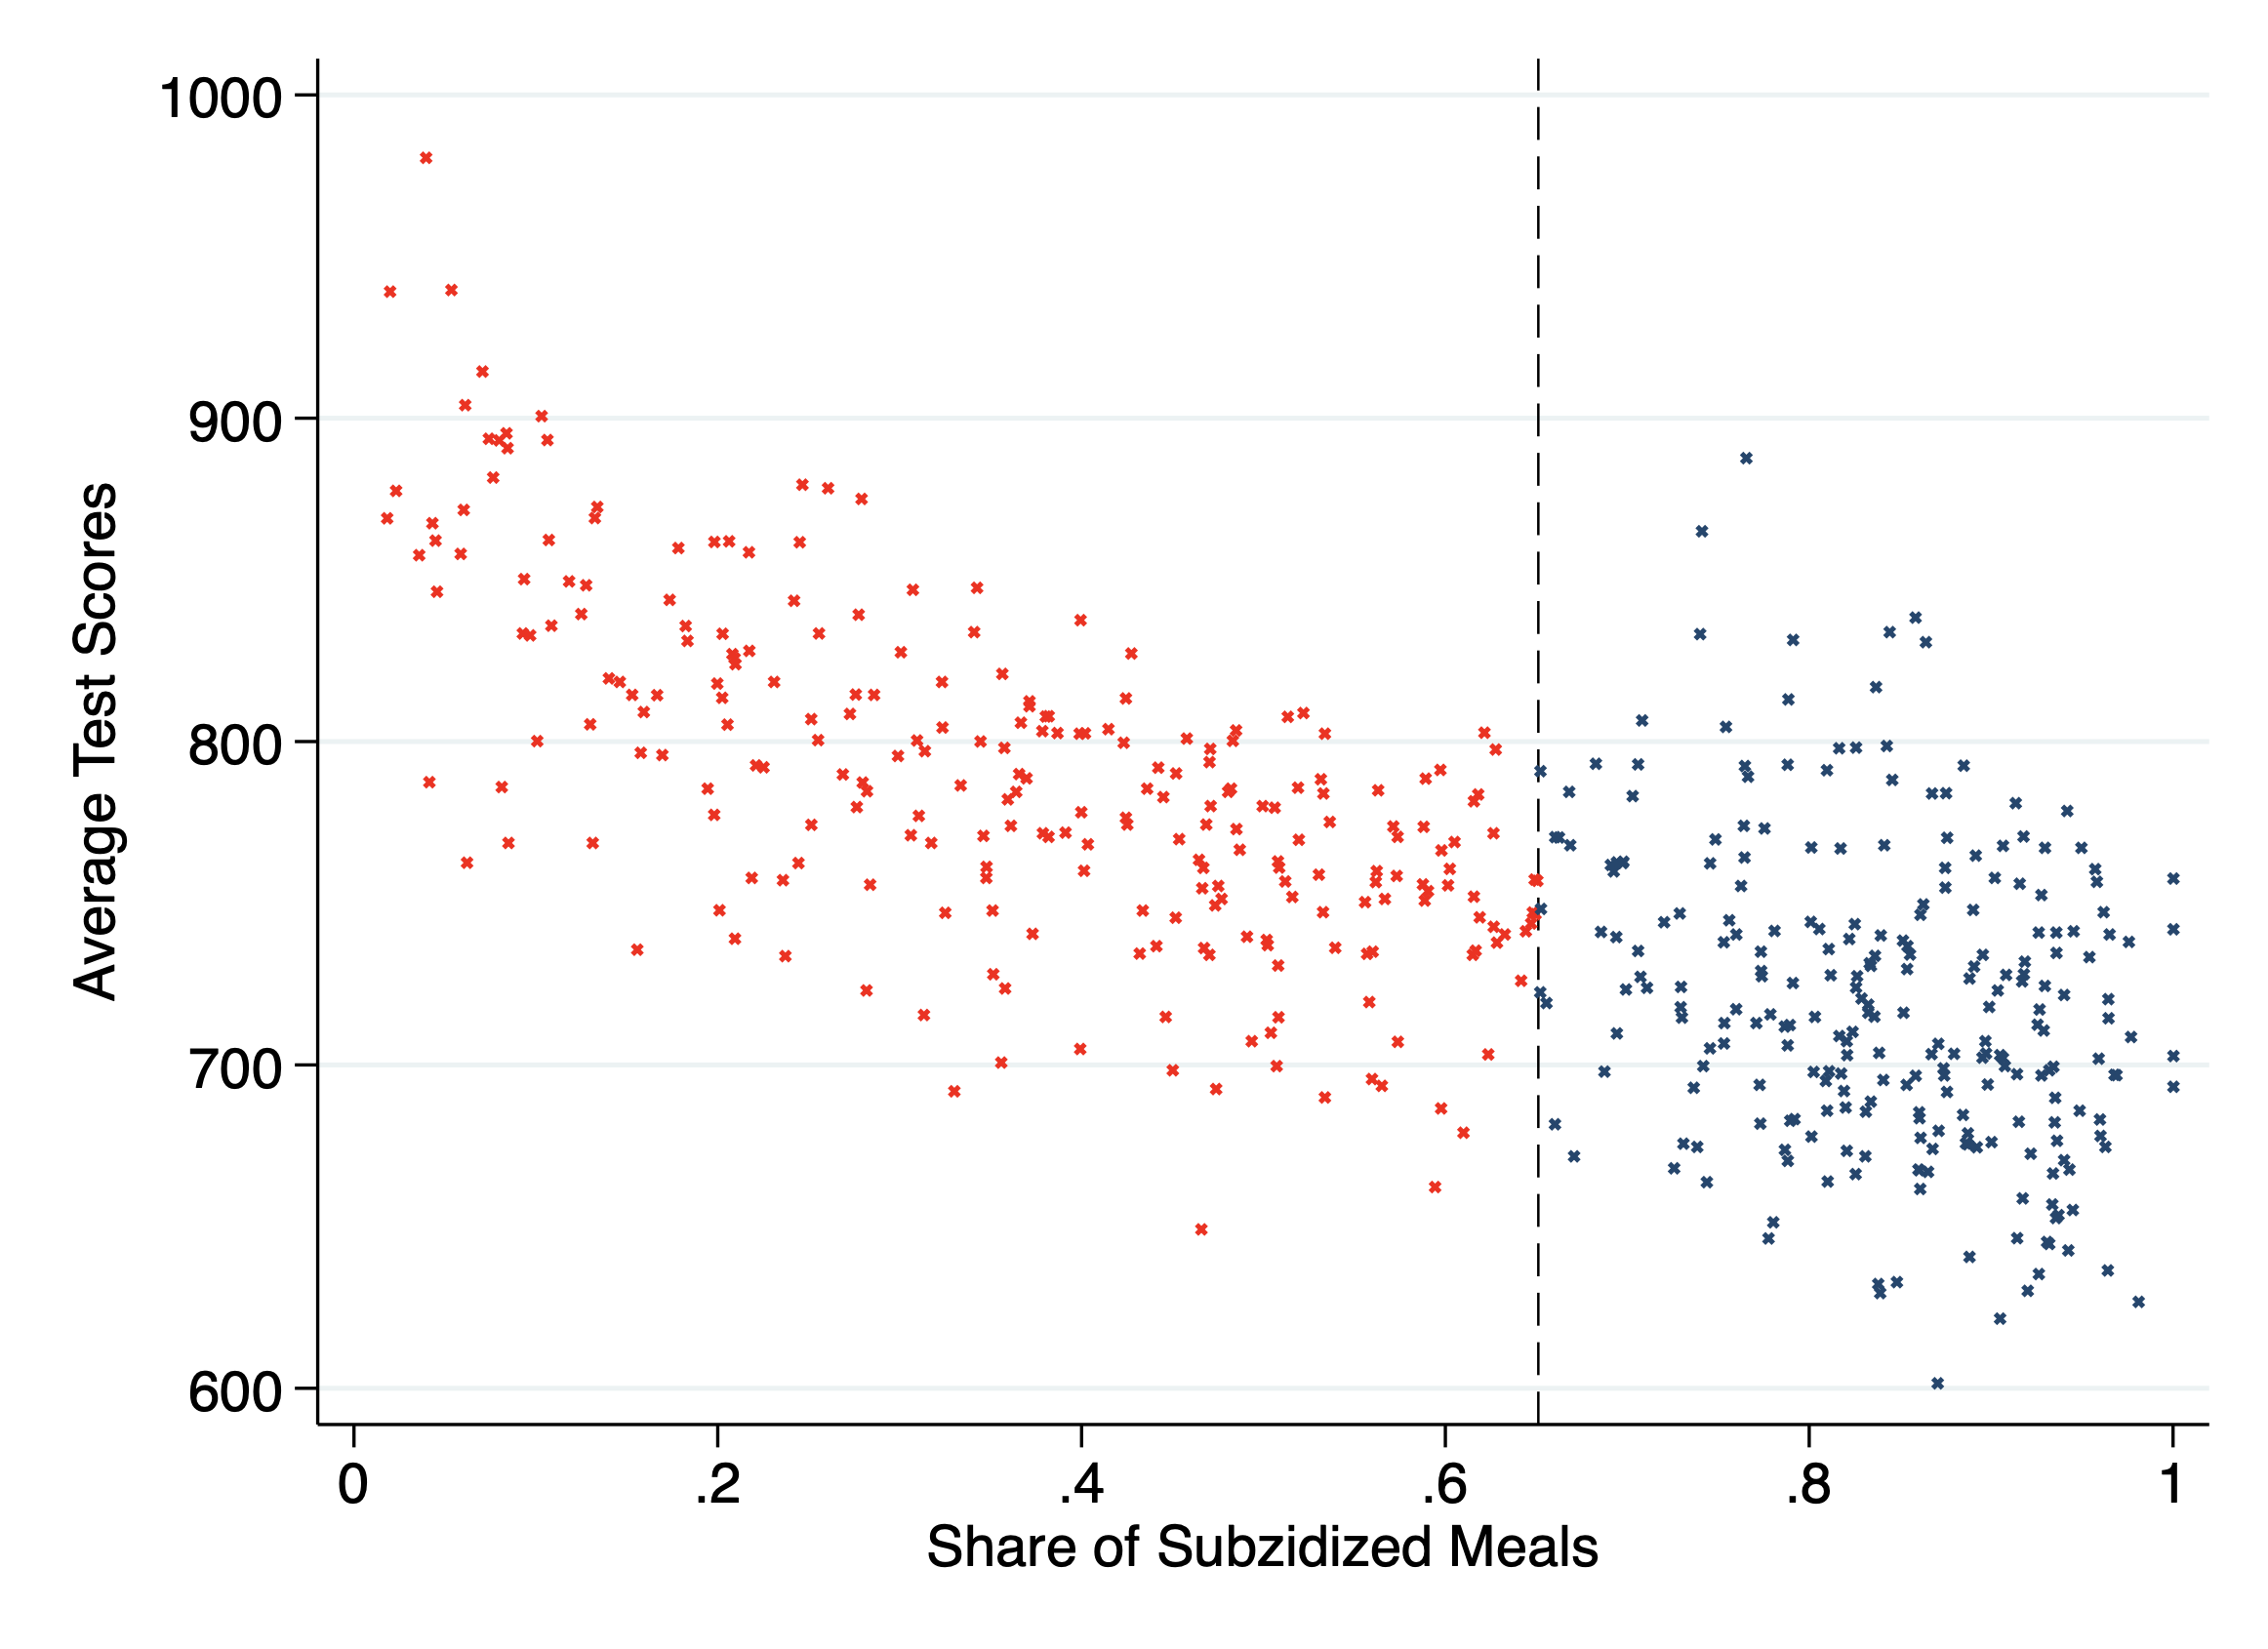
\includegraphics[scale=.25]{images/testscores_group3.png}
\end{figure}
\end{column}
\end{columns}
\end{frame}


\begin{frame}{The California Test Score Data Set}
 \begin{columns}
\begin{column}{0.35\textwidth}
We compute the descriptives for each group
\begin{table}[]
\begin{tabular}{c|c|c|c|}
\cline{2-4}
                            & $\overline{Y}$ & $s^2$ & $n$ \\ \hline
\multicolumn{1}{|c|}{$X^L$} & 787.46         & 52.62 & 250 \\ \hline
\multicolumn{1}{|c|}{$X^H$} & 720.24         & 47.44 & 250 \\ \hline
\end{tabular}
\end{table}
\begin{itemize}
    \item $\overline{Y}^{X^L} - \overline{Y}^{X^H} = 67.214 $
    \item $SE(\overline{Y}^{X^H} - \overline{Y}^{X^L}) =\sqrt{\frac{47.44^2}{250}+\frac{52.62^2}{250}} \approx 4.48 $
    \item $ t =67.214/4.48 \approx 15 > 1.96$
\end{itemize}

\end{column}
\begin{column}{0.7\textwidth}
\begin{figure}
  \centering
         \vspace{-1mm}
        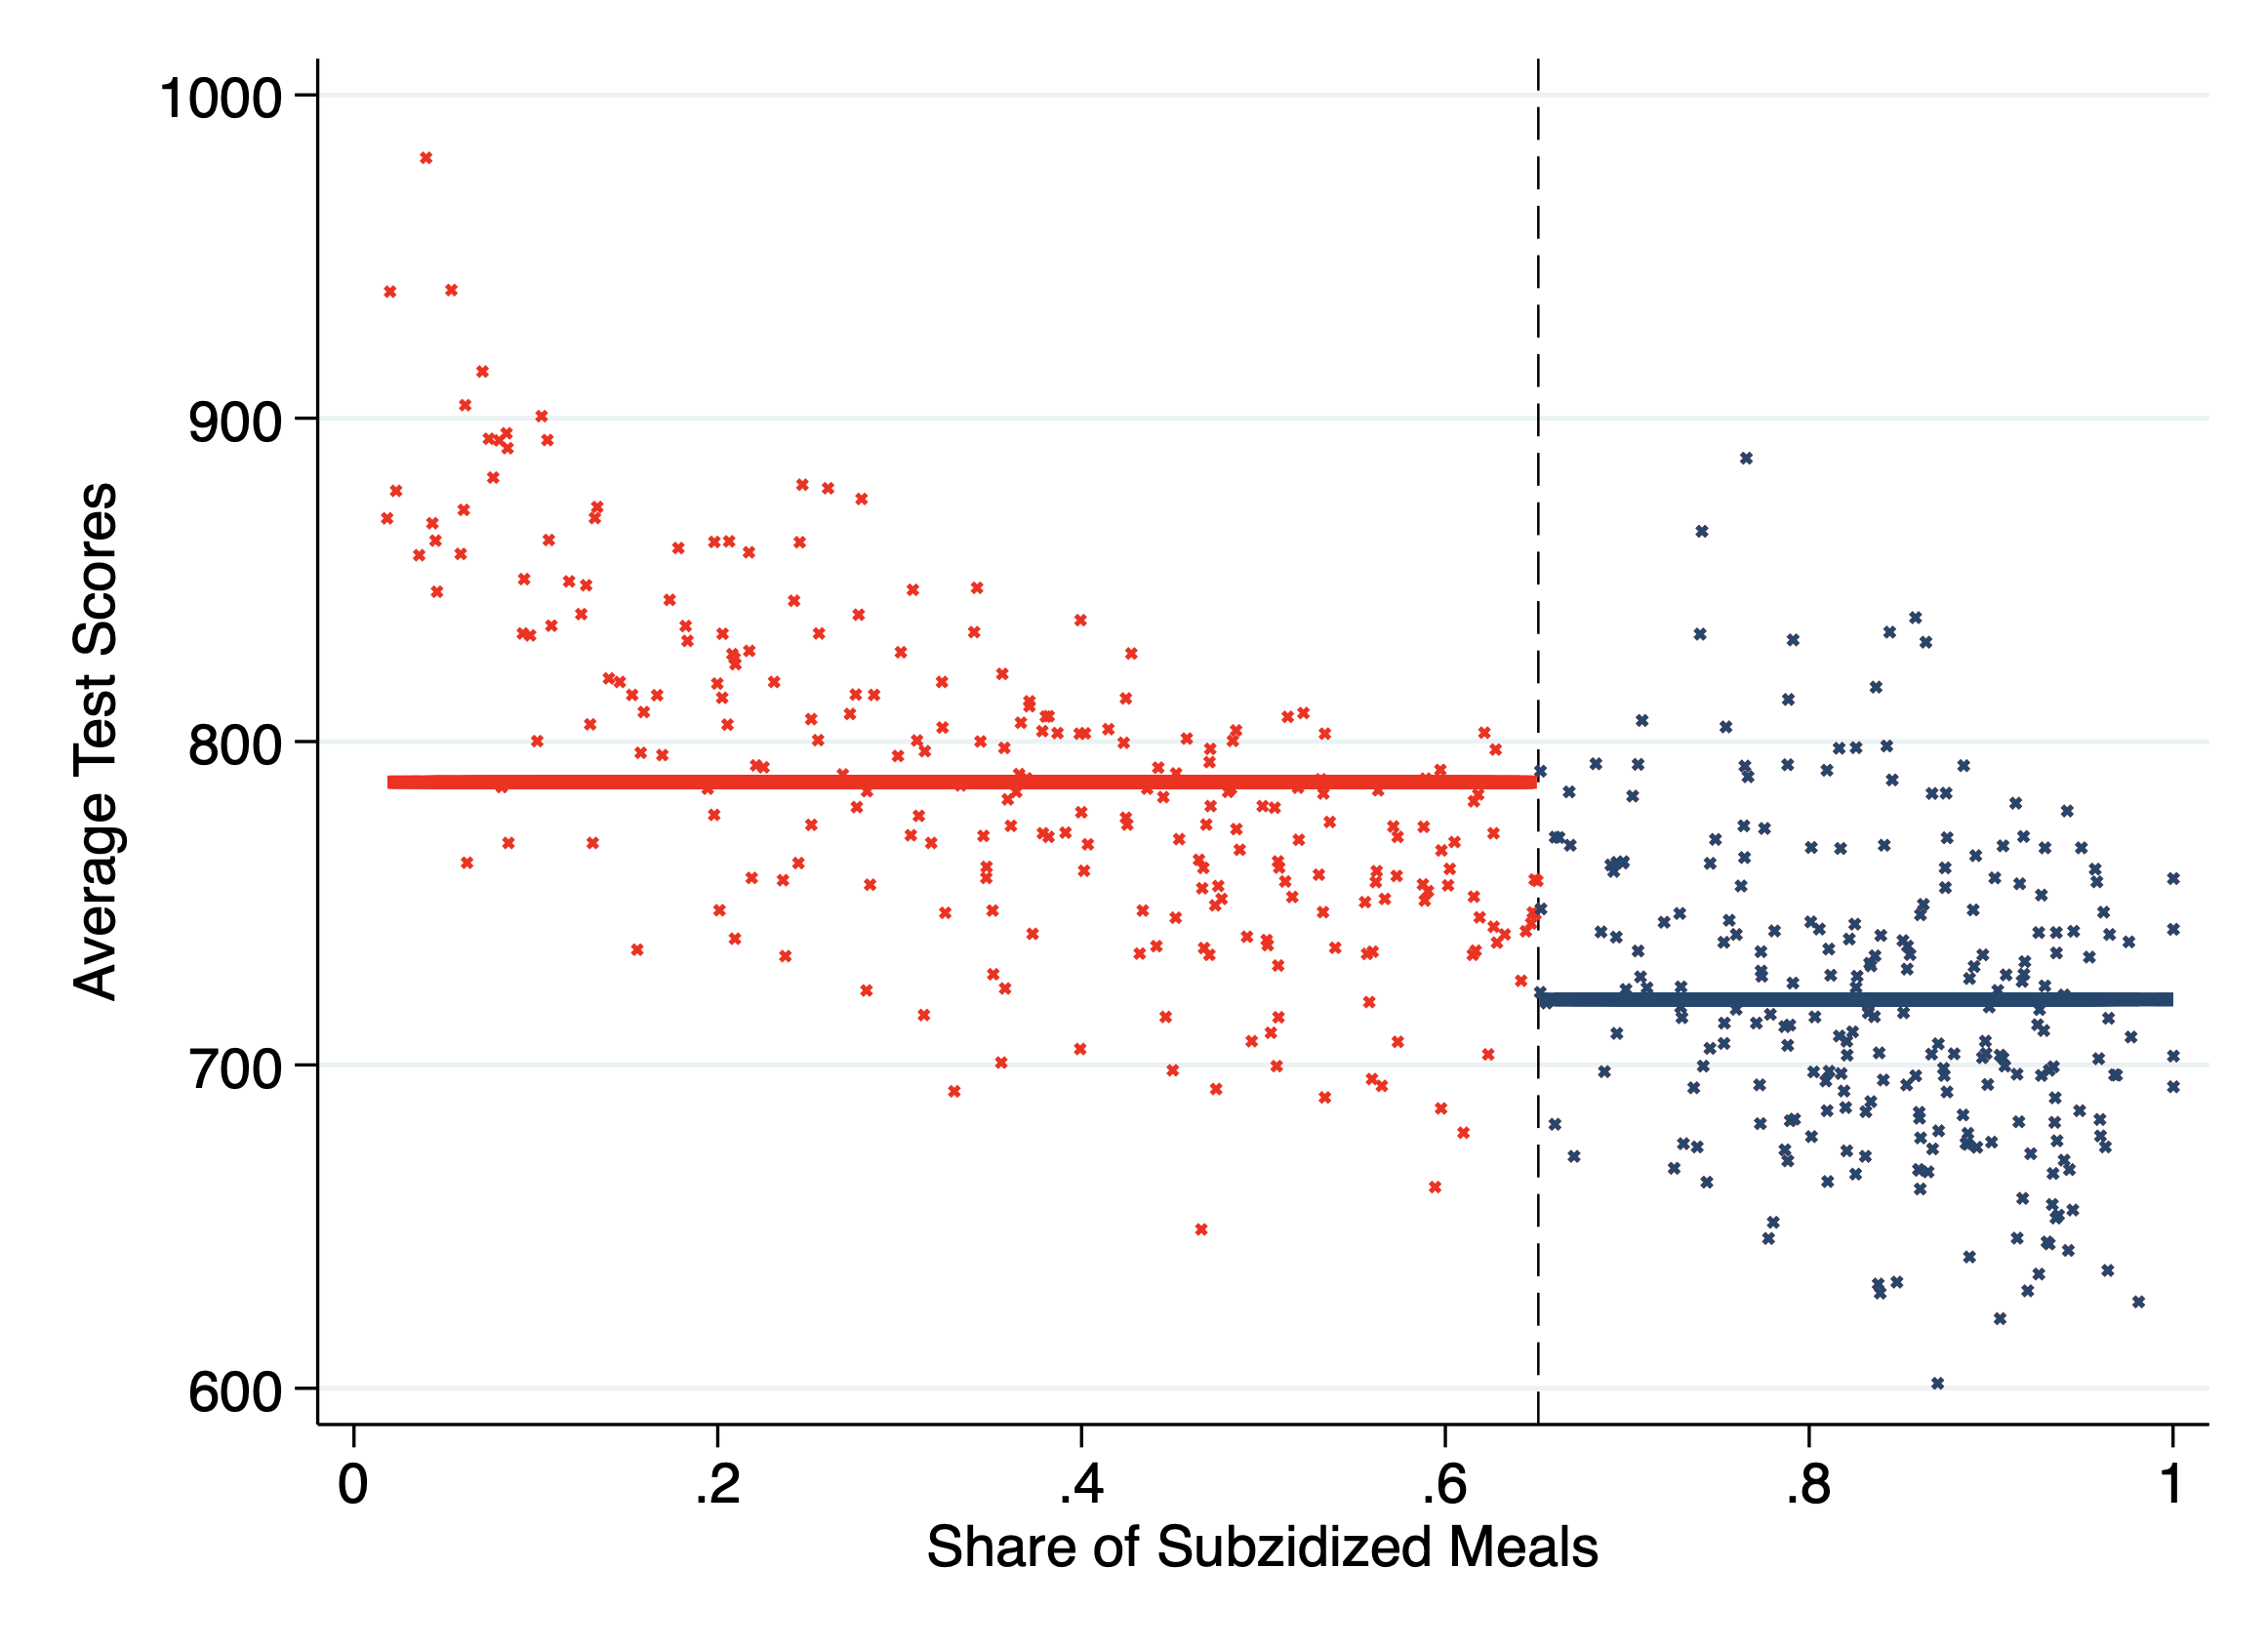
\includegraphics[scale=.25]{images/testscores_group4.png}
\end{figure}
\end{column}
\end{columns}
\end{frame}


\begin{frame}{The California Test Score Data Set}
 \begin{columns}
\begin{column}{0.35\textwidth}
Alternatively, we can also compute the 95\% CI for the difference
\begin{eqnarray*}
    & \overline{Y}^{X^L} &- \overline{Y}^{X^H} \\
    & &\pm 1.96 \times SE(\overline{Y}^{X^H} - \overline{Y}^{X^L})\\
    & &= 67.214 \pm 1.96 \times 4.48\\
    & &= [ 58.41 ; 76.018]\\
    & &\notin 0
\end{eqnarray*}
\begin{itemize}
    \item 
\end{itemize}

\end{column}
\begin{column}{0.7\textwidth}
\begin{figure}
  \centering
         \vspace{-1mm}
        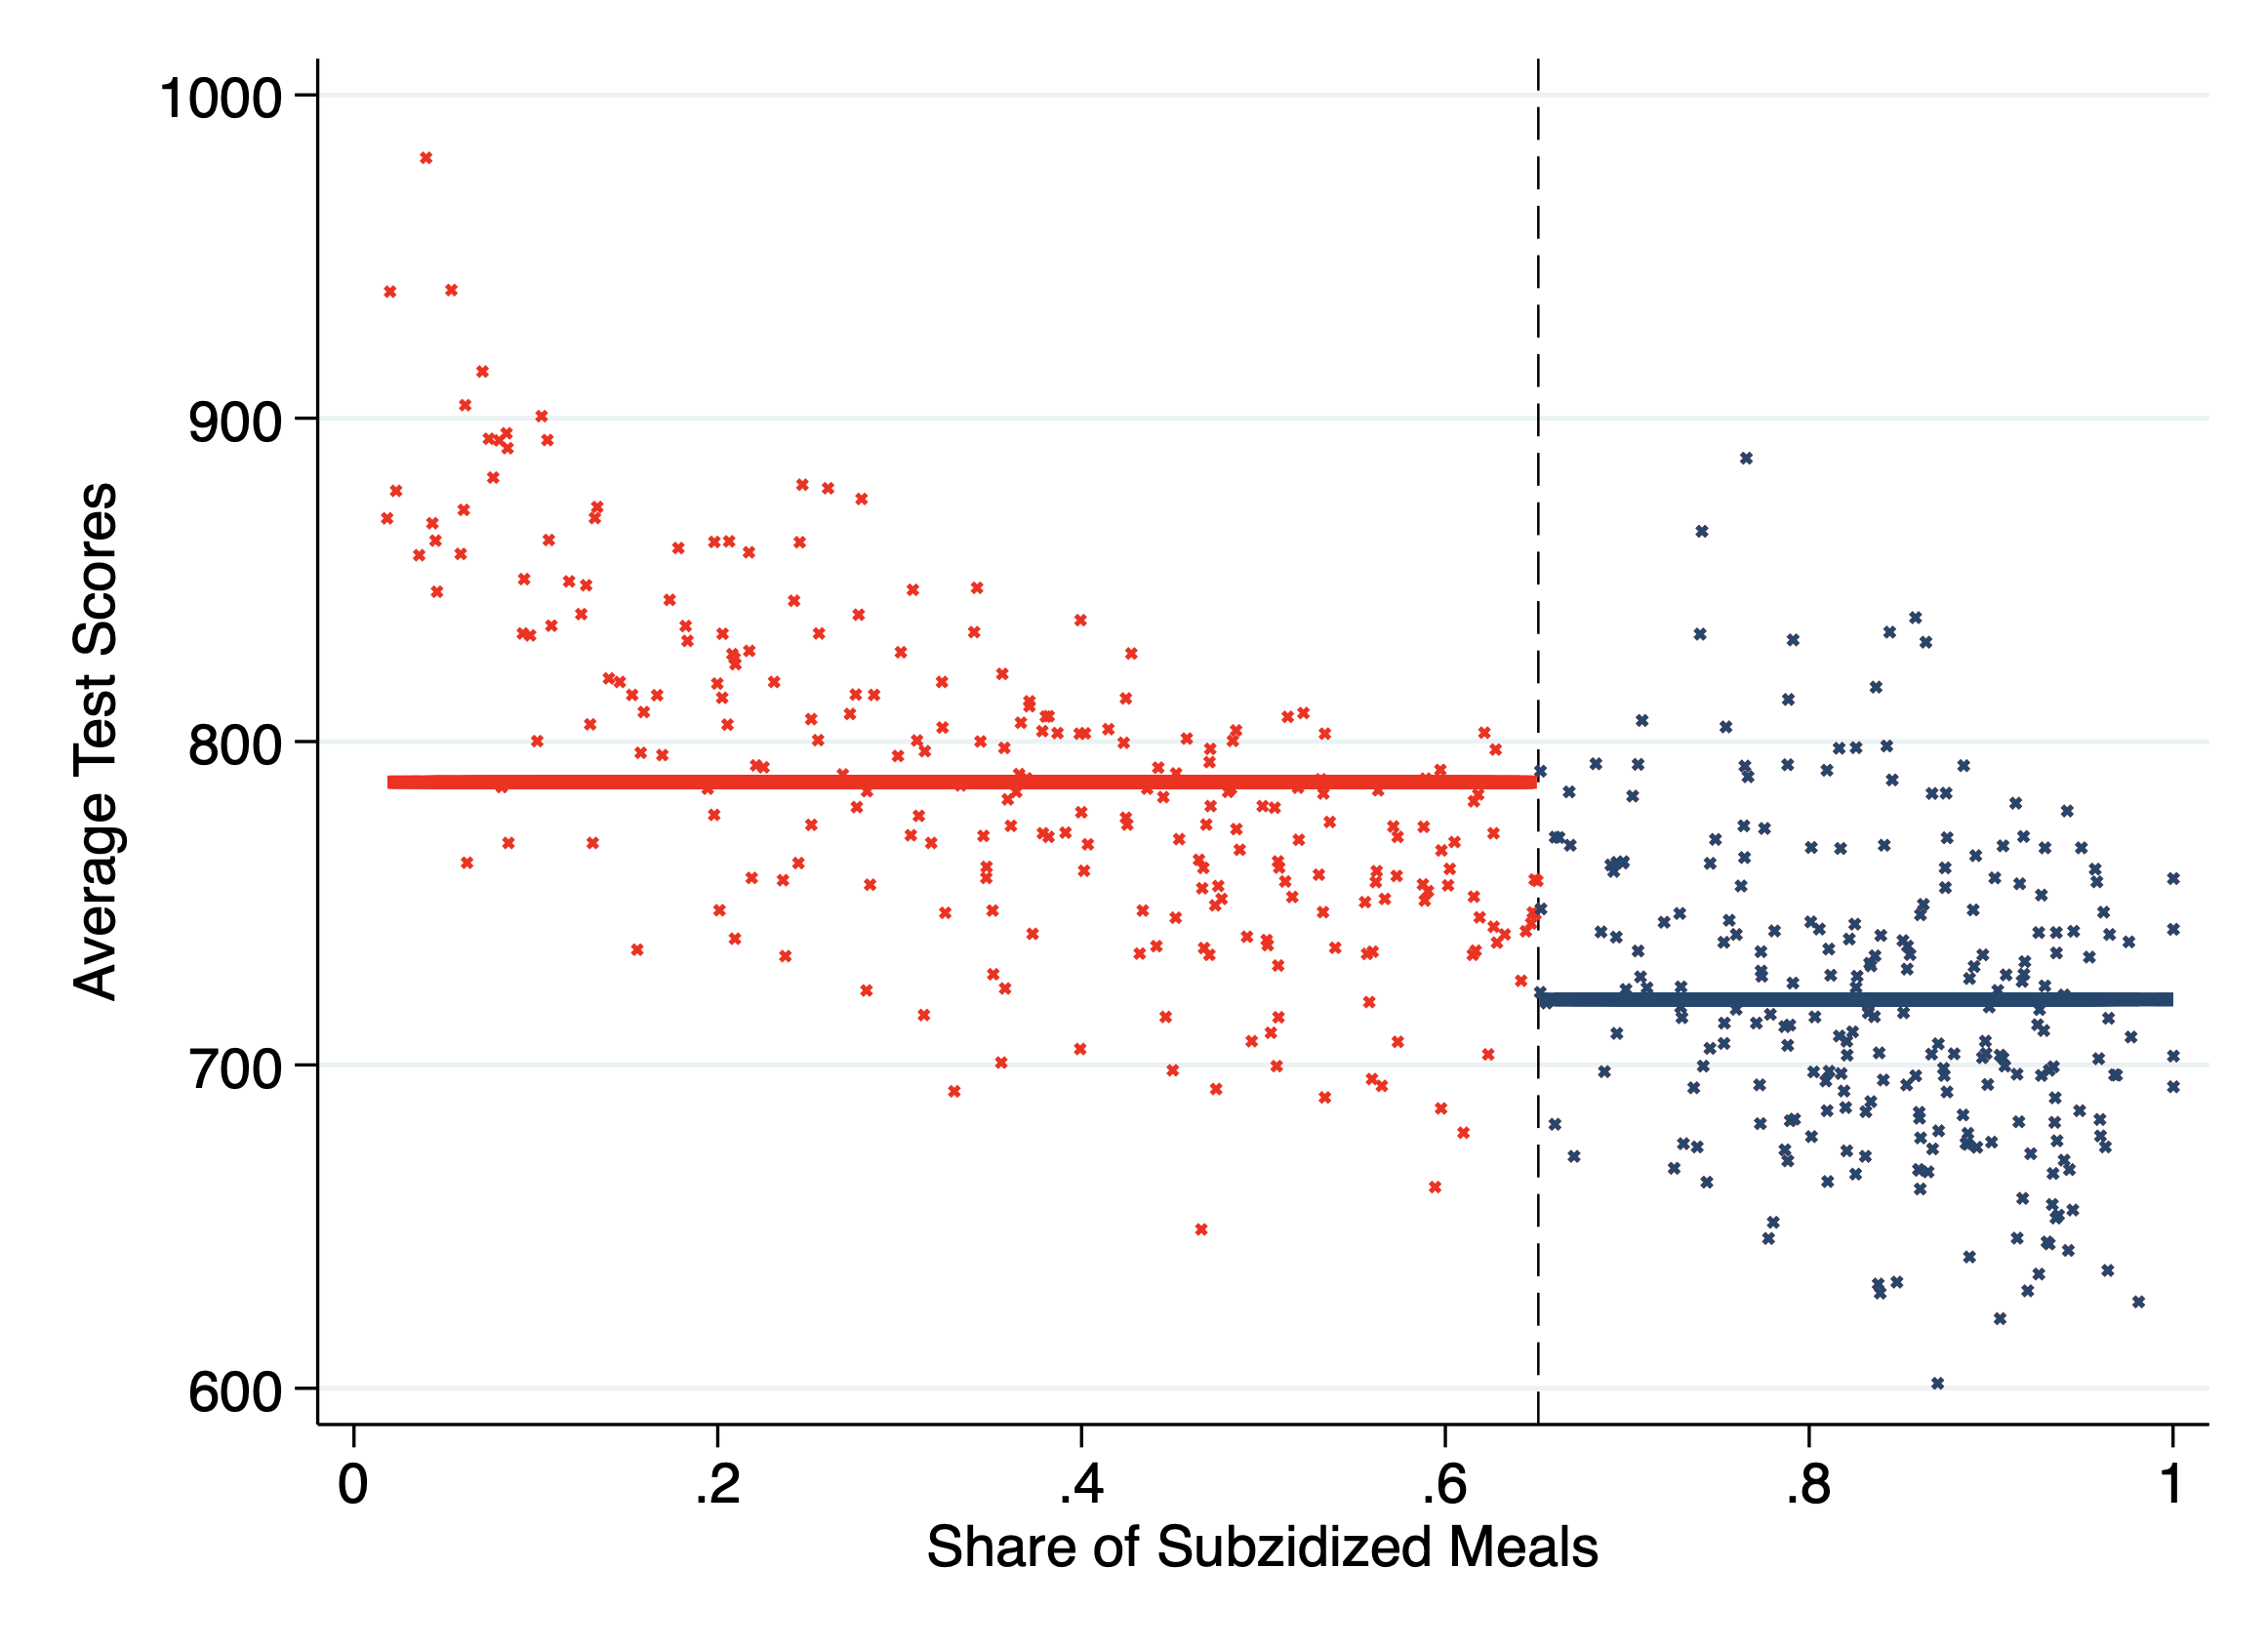
\includegraphics[scale=.25]{images/testscores_group4.png}
\end{figure}
\end{column}
\end{columns}
\end{frame}



\begin{frame}[allowframebreaks]{Material}
\begin{itemize}
    \item[--] \textbf{Textbooks:}
    \begin{itemize}
        \item Introduction to Econometrics, 4th Edition, Global Edition, by Stock and Watson -- Chapter 3
    \end{itemize}
\end{itemize}
\end{frame}



\end{document}
